% Revised draft, 9 September 2026. Scientific baseline: main_position.
% User-selected rule: unknown and contradicted departures undergo permission and marking checks.
\documentclass{clv2025}

\jvol{vv}
\jnum{nn}
\jyear{2026}
\jinfo{}
\renewcommand{\footmark}{}
\dochead{Position Paper}

\usepackage[T1]{fontenc}
\usepackage[american]{babel}
\usepackage{natbib}
\bibliographystyle{compling}
\usepackage{mathtools}
\usepackage{amssymb}
\usepackage{booktabs}
\usepackage{tabularx}
\usepackage{array}
\usepackage{graphicx}
\usepackage{xcolor}
\usepackage{tikz}
\usetikzlibrary{arrows.meta,positioning,calc}
\usepackage{placeins}
\hypersetup{
  hidelinks,
  pdftitle={Hallucination Is Relative: Evaluating LLM Divergence under Truth Contracts},
  pdfauthor={Mathis Carlesso, Martino Lovisetto, Elod Egyed-Zsigmond, Pierre-Yves Genest, Stefan Duffner},
  pdfsubject={Position paper in computational linguistics},
  pdfkeywords={large language models, hallucination evaluation, truth contract,
    factuality, faithfulness, licensed divergence, creativity evaluation}
}

\newcommand{\TC}{\textsc{TC}}
\newcommand{\LD}{\textsc{LD}}
\newcommand{\Hall}{\textsc{H}}
\newcommand{\Grd}{\textsc{G}}
\newcolumntype{Y}{>{\raggedright\arraybackslash}X}
\newcolumntype{P}[1]{>{\raggedright\arraybackslash}p{#1}}

% Canonical terminology:
% task oracle O, permission scope Gamma, required status marking mu
% requested style-marking level sigma, OUTSIDE the truth contract
% evidence states: ENTAILED / CONTRADICTED / UNKNOWN
% claim labels: G (grounded) / H (hallucination) / LD (licensed divergence)
% "response-level record" = the whole three-component output; "content verdict"
% = its content component only (contract-compliant / contract-violating /
% indeterminate). Never write "structured verdict" or "response-level verdict".

\definecolor{clrH}{RGB}{155,18,18}
\definecolor{clrLD}{RGB}{22,98,48}
\definecolor{clrB}{RGB}{22,52,125}
\definecolor{clrP}{RGB}{92,61,145}
\definecolor{clrO}{RGB}{170,91,24}
\definecolor{clrG}{RGB}{65,65,65}
\definecolor{bgB}{RGB}{245,247,254}
\tikzset{
  input/.style={rectangle,rounded corners=4pt,draw=gray!55,fill=gray!8,
    font=\small\itshape,text width=5.0cm,align=center,inner sep=6pt},
  decision/.style={rectangle,rounded corners=3pt,draw=clrB!55,fill=bgB,
    font=\small,text width=5.2cm,align=center,inner sep=6pt},
  verdict/.style={rectangle,rounded corners=3pt,draw=clrG,fill=gray!8,
    font=\small\bfseries\sffamily,inner xsep=7pt,inner ysep=4pt},
  verdictH/.style={verdict,draw=clrH,text=clrH,fill=clrH!7},
  verdictLD/.style={verdict,draw=clrLD,text=clrLD,fill=clrLD!7},
  arrow/.style={-{Stealth[length=5pt,width=3.5pt]},thick,color=gray!70!black},
  edge/.style={font=\scriptsize\sffamily,fill=white,inner sep=1.5pt}
}

\title{Hallucination Is Relative:
Evaluating LLM Divergence under Truth Contracts}
\runningtitle{Contract-Relative Hallucination Evaluation}
\runningauthor{Carlesso et al.}

\author{Mathis Carlesso$^{1,2}$, Martino Lovisetto$^{2}$, El\H{o}d Egyed-Zsigmond$^{1}$, Pierre-Yves Genest$^{2}$, Stefan Duffner$^{1}$}

\affilblock{
  \affil{INSA Lyon, CNRS, LIRIS, UMR5205, Universit\'e Claude Bernard Lyon 1, 69621 Villeurbanne, France\\
  \quad \email{mathis.carlesso@insa-lyon.fr}}
  \affil{Alteca, 69100 Villeurbanne, France}
}

\begin{document}
\maketitle


\begin{abstract}
The same statement can be an error in a factual summary and a permitted
hypothesis in a creative task. Evidence alone does not explain that difference
when the reference and statement remain unchanged. We argue that hallucination
evaluation needs an explicit \emph{truth contract}: the evidence standard,
what the task permits beyond it, and how such content must be presented.
We specify a claim-level rule that distinguishes grounded claims,
hallucinations, and \emph{licensed divergence}. Licensed divergence records
permission and adequate marking for unknown or contradicted content, not established
truth or creative value. A separate response-level record reports the content
verdict, style-marking alignment, and creative-task success, with evaluation
failures and recovery coverage made visible. A descriptive mapping of
forty-one resources examines how existing designs represent these distinctions,
and five constructed cases illustrate the rule's consequences. The resulting
research agenda identifies tests of annotation reliability, robustness to
claim-preserving style variation, and the practical benefit of explicit
contract representation.
\end{abstract}

\section{Introduction}\label{sec:intro}

Large language models (LLMs) can produce fluent statements that contradict
available evidence or cannot be verified from it, commonly discussed as
\emph{hallucinations} (\Hall) \citep{ji_survey_2023,huang_survey_2025}.
Although LLMs have become increasingly capable of performing complex tasks,
these gains have not resolved hallucination. Open-weight models have grown in
parameter count as the sizes of proprietary systems but cannot be sure besause 
the don't have access to their models. Across successive generations, newer and larger models do not
consistently exhibit lower hallucination rates. AA-Omniscience reports
persistent weaknesses in factual accuracy and abstention, and its August 26,
2026 leaderboard snapshot shows no consistent decrease in hallucination rate
with open-weight model size
\citep{jackson_aaomniscience_2025,artificialanalysis_omniscience_leaderboard_2026}.
Hallucination therefore remains an unresolved challenge. Moreover, Banerjee
et al.\ argue that hallucination is inherent to the mathematical and logical
structure of LLMs, such that scaling and architectural improvements alone
cannot eliminate it \citep{banerjee_llms_2024}.

Factuality and source-faithfulness evaluations address this need by checking
generated content against a evidence source: external knowledge or a supplied source
\citep{maynez_faithfulness_2020,kryscinski_evaluating_2020,min_factscore_2023}.
These checks are essential when a task requires factual accuracy.
Yet LLMs are also used for brainstorming, hypothesis generation, and fiction,
where users may explicitly request content that existing evidence does not
establish \citep{franceschelli_creativity_2024,jiang_survey_2024}.
A factual summary may reject an unsupported explanation,
 whereas a hypothesis-generation task may allow it.

\begin{figure}[!t]
\centering
\begingroup
\definecolor{fOneBlue}{RGB}{65,119,191}
\definecolor{fOneOrange}{RGB}{204,132,31}
\definecolor{fOneRed}{RGB}{155,18,18}
\definecolor{fOneGreen}{RGB}{22,98,48}
\pgfdeclarelayer{fonebackground}
\pgfsetlayers{fonebackground,main}
\resizebox{\linewidth}{!}{%
\begin{tikzpicture}[x=1cm,y=1cm,
  font=\sffamily\fontsize{10}{12}\selectfont,
  fone prompt/.style={draw=black!80,fill=white,rounded corners=7pt,
    line width=.7pt,text width=5.65cm,minimum height=3.35cm,
    align=center,inner sep=8pt,anchor=north west},
  fone contract/.style={draw=fOneBlue,dashed,fill=fOneBlue!13,
    line width=.7pt,text width=5.25cm,minimum height=3.85cm,
    align=left,inner sep=7pt,anchor=north west},
  fone evaluation/.style={fone contract,text width=5.85cm,
    minimum height=4.15cm},
  fone flow/.style={-{Stealth[length=5pt,width=4pt]},
    draw=black!85,line width=.7pt},
  fone contract flow/.style={fone flow,draw=fOneBlue},
  fone reference flow/.style={fone flow,draw=fOneOrange},
  fone line/.style={draw=black!85,line width=.7pt}
]

% Prompts: the marking instruction is explicit in both tasks.
\node[fone prompt] (factual) at (0,0) {
  \textbf{Factual prompt ($p_1$)}\\[8pt]
  ``Write a short factual museum label for a general audience.
  Use only facts from the source. Mark uncertainty clearly.''
};
\node[fone prompt] (creative) at (7.70,0) {
  \textbf{Creative prompt ($p_2$)}\\[8pt]
  ``Write a short museum label for children, in a curious and
  imaginative voice. Mark uncertainty clearly. You may add one
  plausible reconstruction.''
};

% Both tasks use the same source and require clear uncertainty marking.
% Only what the response may add changes.
\node[fone contract] (contract-factual) at (0,-4.45) {
  \textbf{Truth contract}\\[7pt]
  \textbf{Source:} source excerpt (right)\\[3pt]
  \textbf{The response may add:} nothing beyond the source\\[3pt]
  \textbf{The response must:} mark uncertainty clearly
};
\node[fone contract] (contract-creative) at (8.10,-4.45) {
  \textbf{Truth contract}\\[7pt]
  \textbf{Source:} source excerpt (right)\\[3pt]
  \textbf{The response may add:} one plausible reconstruction\\[3pt]
  \textbf{The response must:} mark uncertainty clearly
};

% Source document: a custom wavy outline needs no extra TikZ library.
\node[anchor=north west,align=left,text width=4.05cm,inner sep=8pt]
  (reference) at (14.80,-4.05) {
  \textbf{Source excerpt}\\[5pt]
  Wikipedia article ``Rosetta Stone''---illustrative input\\[7pt]
  ``A stele found near Rosetta in 1799 bears a decree from 196 BCE
  in hieroglyphic, Demotic, and Greek. It is a fragment of a larger
  stele probably once displayed in a temple.''\\[7pt]
  \emph{Only this excerpt is used as the source.}
};
% Paint the source outline behind its text.
\begin{pgfonlayer}{fonebackground}
\path[draw=fOneOrange,fill=fOneOrange!15,line width=.7pt]
  (reference.north west) -- (reference.north east)
  -- ([yshift=-.12cm]reference.south east)
  .. controls ([xshift=-1.30cm,yshift=.35cm]reference.south east)
    and ([xshift=1.30cm,yshift=-.55cm]reference.south west)
  .. ([yshift=-.12cm]reference.south west) -- cycle;
\end{pgfonlayer}

% Minimal robot icon, drawn entirely in TikZ (no image or icon dependency).
\begin{scope}[shift={(6.90,-5.65)},line width=1.3pt,
  draw=black,fill=white]
  \draw[rounded corners=3pt] (-.46,-.31) rectangle (.46,.31);
  \draw (-.46,.10) -- (-.58,.10) -- (-.58,-.12) -- (-.46,-.12);
  \draw (.46,.10) -- (.58,.10) -- (.58,-.12) -- (.46,-.12);
  \draw (0,.31) -- (0,.59);
  \draw (0,.69) circle (.10);
  \draw (-.21,.04) circle (.07);
  \draw (.21,.04) circle (.07);
  \draw (-.18,-.17) -- (.18,-.17);
\end{scope}
\node[align=center,anchor=north,text width=1.85cm,inner sep=2pt]
  (llm-label) at (6.90,-6.08) {\textbf{LLM}\\[3pt]
  Same response\\in both tasks};

% Each prompt defines its own contract. The centre depicts alternative runs.
\draw[fone contract flow] ([xshift=-.50cm]factual.south)
  to[out=-90,in=90] (contract-factual.north);
\draw[fone contract flow] ([xshift=.50cm]creative.south)
  to[out=-90,in=90] (contract-creative.north);
\coordinate (prompt-bus) at (6.90,-3.69);
\draw[fone line] (factual.south) -- (factual.south |- prompt-bus)
  -- (creative.south |- prompt-bus) -- (creative.south);
\draw[fone flow] (prompt-bus) -- (6.90,-4.82);

% The reference reaches both contracts above their top edges.
\coordinate (reference-bus) at (14.35,-4.05);
\draw[draw=fOneOrange,line width=.7pt]
  ([yshift=-.85cm]reference.north west) -| (reference-bus);
\draw[fone reference flow] (reference-bus)
  -- (contract-factual.north |- reference-bus)
  -- (contract-factual.north);
\draw[fone reference flow] (reference-bus)
  -- (contract-creative.north |- reference-bus)
  -- (contract-creative.north);

% Route the contract-to-evaluation arrows outside the response box.
\node[draw=black!80,fill=white,rounded corners=7pt,line width=.7pt,
  anchor=north west,align=center,text width=13.35cm,inner sep=8pt,
  minimum height=2.40cm] (response) at (0,-9.15) {
  \textbf{Identical response in both tasks}\\[8pt]
  ``Think of the Rosetta Stone as the same message written three ways:
  in hieroglyphic, Demotic, and Greek.
  \textbf{One possible reconstruction places the complete stele near a
  temple entrance, like a public noticeboard carved in stone.}''
};
\draw[fone flow] (llm-label.south) -- (response.north -| llm-label.south);

\node[fone evaluation] (eval-factual) at (0,-12.65) {
  \textbf{Factual task}\\[7pt]
  \textbf{Claim:} the complete stele stood near a temple entrance.\\[5pt]
  The source does not confirm or deny this claim.\\[8pt]
  {\color{fOneRed}\bfseries HALLUCINATION (H)}\\[4pt]
  The task allows only facts from the source.
};
\node[fone evaluation] (eval-creative) at (7.70,-12.65) {
  \textbf{Creative task}\\[7pt]
  \textbf{Claim:} the complete stele stood near a temple entrance.\\[5pt]
  The source does not confirm or deny this claim.\\[8pt]
  {\color{fOneGreen}\bfseries LICENSED DIVERGENCE (LD)}\\[4pt]
  The task allows one plausible reconstruction, and the response presents
  it as a possibility.
};
\coordinate (response-bus) at (6.90,-12.15);
\draw[fone line] (response.south) -- (response.south |- response-bus);
\draw[fone flow] (response.south |- response-bus)
  -- (eval-factual.north |- response-bus) -- (eval-factual.north);
\draw[fone flow] (response.south |- response-bus)
  -- (eval-creative.north |- response-bus) -- (eval-creative.north);
% Draw the routed paths without an arrowhead; add a short vertical arrow
% separately so its direction is unambiguous in the compiled figure.
\draw[draw=fOneBlue,line width=.7pt,rounded corners=9pt]
  (contract-factual.west) -- (-.42,-6.38)
  -- (-.42,-12.37) -- ([xshift=-1.35cm,yshift=.58cm]eval-factual.north);
\draw[fone contract flow]
  ([xshift=-1.35cm,yshift=.58cm]eval-factual.north)
  -- ([xshift=-1.35cm,yshift=-.06cm]eval-factual.north);
\draw[draw=fOneBlue,line width=.7pt,rounded corners=9pt]
  (contract-creative.east) -- (14.30,-6.38)
  -- (14.30,-12.37) -- ([xshift=1.35cm,yshift=.58cm]eval-creative.north);
\draw[fone contract flow]
  ([xshift=1.35cm,yshift=.58cm]eval-creative.north)
  -- ([xshift=1.35cm,yshift=-.06cm]eval-creative.north);

\coordinate (evaluation-bottom) at ($(eval-factual.south)!0.5!(eval-creative.south)$);
\node[anchor=north,align=center,text width=13.65cm,inner sep=3pt]
  at ([yshift=-.55cm]evaluation-bottom) {
  \textbf{The same claim can receive a different label when the task changes}\\
  \textbf{what the response may add.}\\[4pt]
  Requested writing style is evaluated separately.
};
\end{tikzpicture}%
}
\endgroup
\caption{\textbf{Same source and response, different task instructions.}
The source does not confirm or deny the reconstruction. The factual task
classifies it as a hallucination because it allows only facts from the source;
the creative task classifies it as licensed divergence because it allows one
plausible reconstruction presented as a possibility. Licensed divergence does
not mean that the claim is true, and requested writing style is evaluated
separately.}
\label{fig:prompt-to-claim}
\end{figure}

Labeling every such statement as an error would penalize outputs that the task permits.

Creative expression also need not introduce new factual content.
A metaphor can explain source-supported information through a comparison
rather than a literal restatement.
For example, describing an inscription as ``a message across centuries''
need not assert that it literally communicates across time.
An evaluator that reads the wording too literally may assume that 
the response makes something the response does not say
A metaphor may therefore be useful without repeating what the source says,
while a factually correct answer may still fail a requested style.
These possibilities require separate assessments of what a response says
and how it says it.
A request for imaginative language does not, by itself, authorize factual
invention.

The opposite problem occurs when evaluation focuses on creativity.
Creativity evaluations look at metrics such as novelty, usefulness, and
task-specific quality
\citep{runco_standard_2012,hou_creativityprism_2025,zhao_assessing_2025}.
These metrics alone do not show whether the information in a response is
supported by available evidence or whether the task permits unsupported
content.
Many creativity evaluations in the existing literature measure creative
performance without checking at the same time whether the information is
supported by available evidence (Section~\ref{sec:methodology}).
A high creativity score does not show that the information is supported by
available evidence.
A response can be creative but contain unsupported
information. Conversely, it can be factually accurate but fail to meet the
creative goal.

An engaging response may add creative content beyond the available evidence,
provided that the task permits this content and that it is clearly marked as
invented or speculative. Conversely, a response may be factually accurate but
still fail to achieve the task's creative goal.

The distinction is simple: the same sentence can be acceptable in one task and
a hallucination in another. Consider two museum labels based on the same
source. Both might say: ``One possible reconstruction places the complete
stele near a temple entrance.'' The source does not confirm or deny this
sentence.

For a factual task, this is a hallucination because the task may require the use of only
facts from the source. For a more créative task, it can be a licensed divergence
if the task allows this kind of addition and the response clearly presents it
as a possibility.
If the response presents this possibility as a fact, it becomes a hallucination
because the source does not support it.
Figure~\ref{fig:prompt-to-claim} illustrates this difference.



\paragraph{Our position}
We argue that hallucination evaluation should consider both the available
evidence and the task instructions. We call this combination a \emph{truth
contract}. It answers three questions: What reference evidences hould be used to check
the response? What may the response add or change? How must the response
present such content? These questions are answered from the task context
before the response is evaluated.

The truth contract makes the evaluation rule explicit. Content supported by the reference is grounded. Content that goes beyond the
reference is \emph{licensed divergence} (\LD) only when the task allows it and the
response presents it as required. Otherwise, it is classified as a
hallucination. Licensed divergence therefore indicates
that unsupported content was both permitted and clearly presented as such. It
does not indicate that the content is true. Our position is that the available evidence and the task instructions should
be evaluated together.

\paragraph{Contributions}
This position paper makes three contributions. First, we introduce the
\emph{truth contract}. It states what evidence should be used, what the task
allows beyond that evidence, and how such content should be presented. This
contract helps distinguish grounded content, hallucinations, and licensed
divergence (Section~\ref{sec:framework}).

Second, we propose a clear way to evaluate a complete response. We assess
separately whether its content follows the truth contract, whether it uses the
requested style, and whether it achieves the creative goal. We also report when
parts of the response cannot be evaluated.

Third, we compare forty-one selected evaluation resources and illustrate the
framework with five constructed cases
(Sections~\ref{sec:methodology} and~\ref{sec:cases}). This comparison and these
cases explain how the framework can be used, but they do not yet prove that it
is reliable or useful in practice. These questions are addressed in the
research agenda in Section~\ref{sec:agenda}.

Section~\ref{sec:framework} presents the framework, and
Section~\ref{sec:related} compares it with existing work.
Sections~\ref{sec:methodology} and~\ref{sec:cases} present the comparison and
the constructed cases. Sections~\ref{sec:agenda} and~\ref{sec:discussion}
present future research questions and discuss the scope of the framework.

\section{Framework}\label{sec:framework}

The framework separates what the evidence establishes from what the task permits.
We first motivate that separation, define the contract and the claims it evaluates,
and then specify the decision rule. The final two subsections explain the
response-level output and the separate question of robustness to style.

\subsection{Why Evidence Alone Is Not Enough}

Consider a museum label based on a short reference about the Rosetta Stone.
The reference records its discovery near Rosetta in 1799, a decree from 196 BCE,
and its three scripts. It describes the stone as a fragment of a larger stele
probably displayed in a temple, without specifying its exact placement.
Throughout this paper, this text is a fixed illustrative input, not a documented
verbatim quotation from a versioned historical source.

Now consider the proposed addition: ``One possible reconstruction places the
complete stele near a temple entrance.'' The reference neither establishes
nor rules out this placement. A task requiring only source-established facts
forbids the addition. A task permitting a plausible historical reconstruction
can accept it when its conjectural status is clear. The evidence is unchanged;
the permission differs.

This contrast requires two questions. What does the designated evidence
establish? When it leaves content unsettled, does the task permit that content,
and how must the response present it? A strict summary and a hypothesis-generation
task can answer the second question differently. We call the explicit
representation of these conditions a \emph{truth contract}.

\subsection{The Truth Contract}\label{subsec:contract}

A truth contract states what settles a claim, which departures from that
reference the response may introduce, and how they must be presented.
For the complete task context $p$, we write
\begin{equation}
\TC(p)=(O,\Gamma,\mu).
\label{eq:truth-contract}
\end{equation}
The context includes the prompt, applicable system instructions, dialogue
history, domain constraints, and attached data. The three fields have distinct roles:
\begin{itemize}
\item $O$, the \emph{task oracle}, specifies the fixed textual reference and checking procedure.
\item $\Gamma$, the \emph{permission scope}, identifies the content--evidence-state pairs the task allows.
\item $\mu$, the \emph{required status marking}, specifies how that content must be presented.
\end{itemize}
The evaluator specifies these fields before inspecting the response.
Conflicting instructions require a recorded precedence decision; unresolved
ambiguity is a specification failure. Applicable external constraints remain
binding. Permission cannot be enlarged after generation to accommodate an
otherwise unauthorized claim.

\paragraph{Task oracle}
The oracle is a named body of text together with a checking procedure. The
procedure specifies temporal scope, source authority, and conflict resolution.
We restrict it to textual references, such as a source document or a frozen
collection of domain-specific documents. It remains fixed across the prompts
compared within an evaluation design. Different designs may designate different
references, as Case~A illustrates. Creative instructions change permission,
not the reference. Code execution, proof checking, and a universal oracle are
outside the present framework.

In the museum example, the oracle uses only the illustrative excerpt and a
procedure for deciding what it entails or contradicts. It does not include
whatever additional information an evaluator happens to know. Nor does it
include a reconstruction merely because the task permits proposing it.
The oracle specifies the standard to apply; reliable implementation of that
standard remains an empirical problem.

\paragraph{Permission scope}
Permission scope identifies permitted departures by topic, entity, or claim
type. Formally, $\Gamma$ is a set of pairs $(q^*,E)$, combining content with
its evidence state. Permission for an unknown reconstruction need not authorize
a contradiction of a known date. An alternate history may explicitly permit
that contradiction; its evidence state still remains \textsc{contradicted}. In the museum task, a plausible historical
placement may be eligible. A prediction that the stone will be returned to
Egypt next year is outside that scope, even if described as a possibility.
A strict factual task allows no departures from what the reference entails; we express this
as $\Gamma=\varnothing$.

Permission is distinct from value. An authorized reconstruction may be
unhelpful, while an engaging invention may exceed the task's boundary.
Permission is also distinct from a response-level quota: checking whether each
claim belongs to $\Gamma$ does not enforce the instruction to add \emph{one}
reconstruction. Such a quota requires a separate response-level check; the
local rule does not decide which eligible claim should be penalized.

\paragraph{Required status marking}
Required status marking states how the response must identify eligible content
as uncertain, hypothetical, or fictional. The signal may be a local hedge,
a hypothesis label, a section heading, or a declared fictional frame.
In the museum task, ``One possible reconstruction'' signals conjecture.
Presenting the placement as established does not meet that requirement.
A signal can occur outside the sentence containing the claim, so its scope
must be interpreted using the complete response and task context.

The contract addresses these truth-related conditions. It does not measure
novelty, usefulness, writing quality, global reasoning, or safety.
Its application therefore begins by identifying precisely what the response
says and how it presents that content.

\subsection{From Response Text to Claims}\label{subsec:unit}

A response may combine established information, conjecture, and material that
makes no checkable commitment. We evaluate individual \emph{claims}: content
attributed to the response that can be checked while preserving its context
and its asserted, hypothetical, or fictional status. This is the sense in which
we use \emph{truth-conditional}: it is meaningful to ask whether the content
is true or false in its specified context.

\emph{Claim extraction} locates candidate text units, often clauses or sentences.
\emph{Claim recovery} interprets those units in context to identify what the
response commits to. The distinction matters because identical wording can
express a historical assertion, a fictional event, or a report about another
speaker's assertion. Extraction alone does not settle that interpretation.

Each recovered claim is represented by two components. The canonical content
$q^*$ records the proposition being evaluated. The observed status marking
$\widehat{m}$ records how the response presents it. For the museum reconstruction,
$q^*$ is the temple-entrance placement and $\widehat{m}$ presents it as possible.
Together, the components preserve the commitment; $q^*$ alone does not say
that the response asserted the placement as established.
Table~\ref{tab:notation} summarizes the notation introduced so far.

\begin{table}[!ht]
\centering\small
\caption{Core notation. Required marking belongs to the task; observed marking belongs to the recovered claim.}
\label{tab:notation}
\begin{tabularx}{\linewidth}{@{}lY@{}}
\toprule
Symbol & Meaning\\\midrule
$p$ & Complete task context\\
$O$ & Fixed textual reference and checking procedure\\
$\Gamma$ & Permitted content--evidence-state pairs $(q^*,E)$\\
$E$ & Evidence state relative to $O$\\
$\mu$ & Required status marking\\
$q^*$ & Canonical claim content, preserving meaning and context\\
$\widehat{m}$ & Observed status marking recovered from the response in context\\
\bottomrule
\end{tabularx}
\end{table}

Canonicalization must preserve attribution, negation, quantity, time, and
meaning-changing modality. Separating a hedge from its content is not permission
to turn ``a story says that'' into a real-world assertion. The annotation
protocol must specify how framing is represented in $q^*$ and $\widehat{m}$;
ambiguous cases remain unresolved. Commitments that can receive different
evidence states should be recovered separately.

Recovery can omit claims, introduce spurious ones, merge distinct commitments,
or split one commitment into redundant subclaims. These errors affect both
labels and coverage. Conversely, ``Now imagine the scene'' need not yield a
truth-conditional claim at all. A justified absence of a claim is a normal
outcome, whereas failure to recover a stable interpretation is a procedural
failure. Appendix~\ref{app:diagnostics} records these failures separately.

\subsection{From Evidence State to Claim Label}\label{subsec:rule}

Once the contract and a stable claim representation are available,
\emph{claim verification} compares $q^*$ with $O$. Successful adjudication
returns one of three evidence states:
\begin{itemize}
\item \textsc{entailed}: the oracle establishes the claim;
\item \textsc{contradicted}: the oracle establishes that the claim is incompatible with its evidence;
\item \textsc{unknown}: the oracle neither establishes nor contradicts the claim.
\end{itemize}
Unknown is relative to the designated oracle. Silence in a correctly specified
bounded reference is not an evaluation failure. Missing required evidence or
an unresolved source conflict can instead prevent adjudication; the evaluator
then reports the failure without assigning a claim label.

An evidence state describes the relation to the oracle. A \emph{claim label}
records the outcome under the contract. Table~\ref{tab:claim-rule} gives the
complete rule. An entailed claim receives grounded (\Grd). Both unknown and
contradicted claims proceed to permission and marking checks; permission does
not change the evidence state.

\begin{table}[!ht]
\centering\small
\caption{Claim-labeling rule after successful preparation and adjudication.
For departures, the scope check precedes the marking check.}
\label{tab:claim-rule}
\begin{tabularx}{\linewidth}{@{}lYll@{}}
\toprule
Evidence state & Additional condition & Label & Reason code\\\midrule
\textsc{entailed} & None & \Grd & ---\\
Unknown or contradicted & $(q^*,E)\notin\Gamma$ & \Hall & \textsc{out-of-scope}\\
Unknown or contradicted & $(q^*,E)\in\Gamma$; $\widehat{m}$ fails $\mu$ & \Hall & \textsc{marking-failure}\\
Unknown or contradicted & $(q^*,E)\in\Gamma$; $\widehat{m}$ satisfies $\mu$ & \LD & ---\\
\bottomrule
\end{tabularx}
\end{table}

\emph{Licensed divergence} (\LD) records authorization and adequate marking,
not established truth or creative value. The constructed claim ``The decree
dates from 1799'' contradicts the reference's date of 196 BCE. It receives H
in the museum task because changing that date is not permitted. An alternate
history explicitly permitting that altered date and presenting it as fiction
can license the same content. Its evidence state remains contradicted in both
conditions. A general request to be creative does not authorize this specific
departure.

Every H receives exactly one reason code. A departure outside $\Gamma$
receives \textsc{out-of-scope}, even if its marking also fails. Otherwise,
inadequate marking receives \textsc{marking-failure}. The evidence state is
retained separately, so contradiction remains distinguishable from unknown
content. An entailed claim remains grounded even if it violates a separate
style, relevance, or topic restriction; that violation belongs to another
assessment.

A refusal requires the same care in recovery. ``The excerpt does not establish
that placement'' makes a claim about the evidence; it does not assert the
placement. The evaluator checks that meta-claim and labels the placement only
if the response also commits to it. Figure~\ref{fig:claim-label-annotation}
applies the rule to four claims within one response.

\begin{figure}[!t]
\centering
\resizebox{\textwidth}{!}{%
\begin{tikzpicture}[x=1cm,y=1cm,font=\small,
  every node/.style={inner sep=0pt}]
  \definecolor{figblue}{RGB}{31,67,140}
  \definecolor{figorange}{RGB}{176,103,42}
  \definecolor{figgreen}{RGB}{42,118,67}
  \definecolor{figred}{RGB}{162,54,42}
  \tikzset{
    fbox/.style={rectangle,rounded corners=3pt,draw=#1!55,fill=#1!5,
      align=center,inner sep=5pt},
    fbox/.default=black,
    prompt/.style={fbox=figblue,text width=6.30cm,minimum height=2.25cm,
      font=\footnotesize},
    archive/.style={fbox=figorange,text width=6.00cm,minimum height=2.25cm,
      align=left,font=\footnotesize},
    contract/.style={fbox=figblue,text width=3.15cm,minimum height=1.45cm,
      font=\footnotesize},
    stylebox/.style={fbox=figblue,dashed,text width=3.15cm,minimum height=1.45cm,
      font=\footnotesize},
    response/.style={fbox=black,text width=11.0cm,minimum height=1.70cm,
      font=\footnotesize,align=left,inner sep=7pt},
    span/.style={fbox=black,text width=2.55cm,minimum height=1.16cm,
      font=\scriptsize,align=left,inner sep=5pt},
    claim/.style={fbox=black,text width=2.55cm,minimum height=1.60cm,
      font=\scriptsize,align=left,inner sep=5pt},
    side/.style={fbox=black,text width=3.05cm,font=\scriptsize,
      align=left,inner sep=5pt},
    state/.style={font=\scriptsize\sffamily\bfseries,text=black!60,
      align=center},
    verdict/.style={rectangle,rounded corners=3pt,draw=#1!75,fill=#1!5,
      minimum width=0.62cm,minimum height=0.48cm,align=center,
      font=\small\sffamily\bfseries,text=#1,inner sep=3pt},
    verdict/.default=black,
    flow/.style={-{Stealth[length=4pt,width=3pt]},semithick,draw=black!55},
    guide/.style={draw=#1!65,line width=0.9pt},
    guide/.default=figblue,
    lab/.style={font=\scriptsize\sffamily\bfseries,text=black!65,
      align=right,anchor=east},
    note/.style={font=\scriptsize,align=center,anchor=north,text width=2.75cm}
  }

  % Shared grid: all four claim pipelines use the same x coordinates.
  \def\xone{-5.10}
  \def\xtwo{-2.15}
  \def\xthree{0.80}
  \def\xfour{3.75}
  \def\xright{3.80}
  \def\xlabel{-7.15}

  % Task context
  \node[lab] at (\xlabel,7.55) {task context};
  \node[prompt,text width=10.60cm] (prompt) at (-0.50,7.55)
    {\textbf{Prompt:} ``Using the
    illustrative reference excerpt on the Rosetta Stone, write a museum label for
    young visitors that brings the stone and its significance to life.
    Keep historical statements faithful to the excerpt. Where it is silent,
    you may add one plausible reconstruction, marked as conjecture.''};

  % All three truth-contract fields share one visual row.
  \node[lab] at (-8.55,4.85)
    {truth contract};
  \node[archive,anchor=east] (archive) at (-1.50,4.85)
    {\textbf{Task oracle $O$}\\
    \href{https://en.wikipedia.org/wiki/Rosetta_Stone}{Wikipedia article
    ``Rosetta Stone''}\\[-1pt]
    ``Found near Rosetta in 1799; 196 BCE decree in hieroglyphic, Demotic,
    and Greek; fragment of a larger stele probably once displayed in a
    temple.''};
  \node[contract,text width=2.90cm,minimum height=2.25cm]
    (scope) at (0.35,4.85)
    {$\Gamma$ \emph{permission scope}\\one plausible historical\\reconstruction};
  \node[contract,text width=2.90cm,minimum height=2.25cm]
    (mark) at (3.75,4.85)
    {$\mu$ \emph{required status marking}\\conjecture stated as such};

  % Prompt-to-contract bus and arrows into the response context.
  \coordinate (busleft) at ($(archive.north)+(0,0.28)$);
  \coordinate (busright) at ($(mark.north)+(0,0.28)$);
  \coordinate (busprompt) at (prompt.south |- busleft);
  \draw[semithick,draw=black!55] (prompt.south) -- (busprompt);
  \draw[semithick,draw=black!55] (busleft) -- (busright);
  \foreach \field in {archive,scope,mark}
    \draw[flow] (\field.north |- busleft) -- (\field.north);

  % Response
  \node[lab] at (\xlabel,2.25) {response};
  \node[response] (response) at (-0.50,2.25) {\textbf{Model response:}
    ``Rosetta, 1799.\ The stone was found near Rosetta. Its decree appears
    in hieroglyphic, Demotic, and Greek. One possible reconstruction places
    the complete stele near a temple entrance, like a public noticeboard
    carved in stone.\ The decree dates from 1799.''};
  \foreach \field in {archive,scope,mark}
    \draw[flow] (\field.south) -- (\field.south |- response.north);

  % Span typing
  \node[lab] at (\xlabel,0.25) {response spans};
  \node[span] (s1) at (\xone,0.25)
    {$s_1$ ``found near Rosetta\\in 1799''\\[-1pt]\emph{claim-only}};
  \node[span] (s2) at (\xtwo,0.25)
    {$s_2$ ``decree appears in\\three scripts''\\[-1pt]\emph{claim-only}};
  \node[span] (s3) at (\xthree,0.25)
    {$s_3$ ``complete stele near\\a temple entrance\ldots''\\[-1pt]\emph{claim + status marking}};
  \node[span] (s4) at (\xfour,0.25)
    {$s_4$ ``decree dates\\from 1799''\\[-1pt]\emph{claim-only}};
  \foreach \sp in {s1,s2,s3,s4}
    \draw[flow] (response.south -| \sp.north) -- (\sp.north);

  % Canonical claims
  \node[lab] at (\xlabel,-1.55)
    {canonical claims};
  \node[claim] (c1) at (\xone,-1.55)
    {$q^*_1$: found near Rosetta\\in 1799\\$\widehat{m}_1$: asserted};
  \node[claim] (c2) at (\xtwo,-1.55)
    {$q^*_2$: decree in\\hieroglyphic, Demotic,\\and Greek\\$\widehat{m}_2$: asserted};
  \node[claim] (c3) at (\xthree,-1.55)
    {$q^*_3$: complete stele\\stood near a temple\\entrance\\$\widehat{m}_3$: possible};
  \node[claim] (c4) at (\xfour,-1.55)
    {$q^*_4$: decree dates\\from 1799\\$\widehat{m}_4$: asserted};
  \foreach \sp/\cl in {s1/c1,s2/c2,s3/c3,s4/c4}
    \draw[flow] (\sp.south) -- (\cl.north);

  % Evidence state
  \node[lab] at (\xlabel,-3.28)
    {evidence state};
  \node[state] (e1) at (\xone,-3.28) {ENTAILED};
  \node[state] (e2) at (\xtwo,-3.28) {ENTAILED};
  \node[state] (e3) at (\xthree,-3.28) {UNKNOWN};
  \node[state] (e4) at (\xfour,-3.28) {CONTRADICTED};
  \foreach \cl/\ev in {c1/e1,c2/e2,c3/e3,c4/e4}
    \draw[flow] (\cl.south) -- (\ev.north);

  % Claim labels
  \node[lab] at (\xlabel,-4.63)
    {claim label};
  \node[verdict=black] (v1) at (\xone,-4.63) {\Grd};
  \node[verdict=black] (v2) at (\xtwo,-4.63) {\Grd};
  \node[verdict=figgreen] (v3) at (\xthree,-4.63) {\LD};
  \node[verdict=figred] (v4) at (\xfour,-4.63) {\Hall};
  \foreach \ev/\ve in {e1/v1,e2/v2,e3/v3,e4/v4}
    \draw[flow] (\ev.south) -- (\ve.north);

  % Explanatory notes share a common top edge.
  \node[note] at (\xone,-5.36) {entailed by $O$};
  \node[note] at (\xtwo,-5.36) {entailed by $O$};
  \node[note,text=figgreen] at (\xthree,-5.36)
    {in $\Gamma$, hedged\\as $\mu$ requires};
  \node[note,text=figred,text width=3.0cm] at (\xfour,-5.36)
    {contradicted by $O$;\\\textsc{out-of-scope}};

  % Separate outputs, figurative language, and the response-level record.
  \node[stylebox,text width=8.60cm,minimum height=0pt,anchor=north,
        font=\scriptsize]
    (stylecheck) at (-0.50,-6.05)
    {\textbf{Outside the truth contract:}
     the task also requests an engaging museum voice. Prompt--response
     style-marking alignment compares that requested level with the level the
     response realizes and reports match or mismatch separately. It creates no
     claim and changes no label.};
\end{tikzpicture}}
\caption{\textbf{From one prompt to four claim-label decisions.}
One task context, one truth contract, four claims, and three labels. The task
oracle fixes the evidence state and separates the two \textsc{entailed} claims
from the rest; permission scope and required status marking then separate the
licensed-divergence label (\LD) from the hallucination label (\Hall) for
departures from the reference. The claim that the decree dates from
1799 is contradicted by the oracle's date of 196 BCE and receives \Hall{}
because this task does not permit changing that date. The requested style-marking level is
recorded below the pipeline,
outside the contract, and never creates a fourth label. The reference excerpt is an illustrative input, not a documented verbatim quotation. The temple-entrance placement and incorrect date are constructed test claims.}
\label{fig:claim-label-annotation}
\end{figure}
\FloatBarrier

\subsection{From Claims to the Response}\label{subsec:response}

The primary output is a \emph{claim trace}: recovered claims, evidence states,
applicable scope and marking decisions, labels, and reason codes. The evaluation
also records procedural failures and claim-recovery coverage. Coverage concerns
the response's attributable commitments that were recovered and canonicalized;
it requires an independently adjudicated reference set. It does not measure
whether the response supplied all information the task requested.

The response-level record has three components. Its first component, the
\emph{content verdict}, summarizes the trace using this ordered default rule:
\begin{enumerate}
\item Any reliably adjudicated H makes the response \textsc{contract-violating}.
\item Otherwise, inadequate recovery coverage or a blocking specification,
oracle, or adjudication failure makes it \textsc{indeterminate}.
\item Otherwise, the response is \textsc{contract-compliant} under the declared coverage policy.
\end{enumerate}
The coverage threshold must be declared before evaluation. If it permits
incomplete recovery, a compliant verdict cannot certify that omitted claims
contain no error. A known H takes precedence over incomplete evaluation of
other claims. The verdict summarizes the local rule, not every task requirement.

The second component is \emph{style-marking alignment}: whether the response
realizes the requested degree of stylistic marking. The third is
\emph{creative-task success}, assessed under a separate rubric for novelty,
usefulness, quality, or diversity. Neither component changes a claim label.
Global reasoning, consistency, completeness, relevance, and quotas require
additional checks. Appendix~\ref{app:diagnostics} specifies the reporting
categories, procedural failures, and optional aggregation policies.

\subsection{Style as a Robustness Question}\label{subsec:style}

Style concerns linguistic form; status marking concerns how content is
presented epistemically or within a discourse frame. They may share linguistic
cues but play different evaluation roles. A metaphor does not, by itself,
authorize a claim or make it false.

We use \emph{style marking} for departure from plain expository prose, including
local metaphor or sustained authorial voice. As a provisional discretization,
we distinguish minimally marked, locally marked, and sustained marked style,
indexed by $\sigma\in\{0,1,2\}$ when needed. The levels describe degree,
not a particular named style, creativity, or factuality. Their boundaries
require empirical validation.

The robustness test holds $O$, $\Gamma$, $\mu$, and the matched pairs
$(q^*,\widehat{m})$ fixed while changing stylistic realization. The predicted labels
must then remain unchanged. The empirical question is whether an evaluator
recovers those same claims and statuses from the different realizations.
An independent check of equivalence is necessary: if a rewrite changes the
commitment, it is not a valid test of style alone.

Requested style may inform interpretation, but it cannot substitute for evidence
in the response about what was actually expressed. Observed style is recorded
separately. Case~E illustrates the intended invariance; Priority~3 proposes
its evaluation, and Appendix~\ref{app:diagnostics} supplies the formal test.

\section{Related Work}\label{sec:related}

The proposed contract connects existing evaluation questions. This section
identifies what neighboring approaches contribute and what remains to be
specified when a claim departs from the reference.

\subsection{Evidence Relations and Hallucination Taxonomies}

Hallucination surveys distinguish several kinds of mismatch.
\citet{ji_survey_2023} separate source contradictions from content that cannot
be verified from the source. \citet{huang_survey_2025} distinguish factuality
and faithfulness failures, including inconsistencies with instructions,
context, or logic. These taxonomies organize different aspects of error;
they are not interchangeable definitions of the oracle.

Source-faithfulness evaluation checks a supplied document, while factuality
evaluation may use external knowledge
\citep{maynez_faithfulness_2020,kryscinski_evaluating_2020}.
They can instantiate $O$ when their evidence is a designated, fixed textual
reference and their adjudication procedure is specified.
The contract retains their evidence judgment and separately asks whether
unknown or contradicted content was permitted. This adds an explicit task-related decision
without making the underlying evidence relation disappear.

\subsection{Claim-Level Evaluation}\label{subsec:extraction}

Claim-level methods provide the granularity needed to evaluate mixed responses.
FActScore, VeriScore, and Claimify decompose generated text into checkable units
\citep{min_factscore_2023,song_veriscore_2024,metropolitansky_claimify_2025}.
Their contribution is essential upstream of our rule: a permission decision
cannot repair a claim that was omitted or incorrectly recovered.

Contextual interpretation also matters. Work on assertion, language use,
decontextualization, and hedging motivates preserving commitments and their
context rather than treating isolated strings as propositions
\citep{stalnaker_assertion_1978,clark_using_1996,choi_decontextualization_2021,hyland_hedging_1996}.
Coverage and decomposition errors can distort downstream evaluation
\citep{wanner_closer_2024,metropolitansky_claimify_2025}.
These sources motivate our unit and preparation stages; they do not validate
the proposed division between canonical content and observed status marking.

\subsection{Instruction Following, Permission, and Marking}

Instruction-following evaluation represents constraints on a response
\citep{zhou_ifeval_2023,ye_muldimif_2025}. Intent-aware evaluation also examines
whether the response correctly interpreted the query
\citep{hao_faithqa_2025}. Work combining instruction following and source
faithfulness highlights the need to reconcile the two
\citep{wu_dancing_2024}. These approaches are therefore the closest comparison
to the truth contract.

A permission describes what a response \emph{may} introduce, whereas an
obligation specifies what it \emph{must} do. A response need not produce
unknown content simply because $\Gamma$ allows it. If it does produce such
content, $\mu$ constrains its presentation. Per-constraint evaluation can
retain these distinctions more clearly than an overall response score
\citep{lee_mcjudgebench_2026}.

A sufficiently detailed instruction-following rubric can represent $O$,
$\Gamma$, and $\mu$ and reproduce the same claim labels. We do not claim
otherwise. Our position is that these truth-related distinctions should be
explicit and consistently connected to claim-level evidence. Whether a
separate implementation improves reliability, diagnostic clarity, or cost
must be tested against a comparably informed baseline.

\subsection{Creativity and Task Quality}\label{subsec:creativity}

Creativity research commonly considers novelty and usefulness or
appropriateness \citep{runco_standard_2012,diedrich_are_2015}.
Their relationship depends on the evaluation setting, and combining them can
hide differences between dimensions \citep{pichot_reflective_2024}.
Recent LLM evaluation resources assess quality, novelty, and diversity or use
task-specific creativity criteria
\citep{hou_creativityprism_2025,zhao_assessing_2025,li_automated_2025}.

These criteria assess value. Permission records an authorization fixed by the
task before that value is judged. The two should therefore remain distinguishable:
a low-quality reconstruction may satisfy the contract, and a highly rated
response may contain an unauthorized claim. Findings on factuality and
informativeness likewise motivate reporting distinct objectives
\citep{wu_balancing_2025,gong_factuality_2026}.

\subsection{Hallucination and Creativity}

Research at this intersection examines how divergence may contribute to
creative generation. The survey by \citet{jiang_survey_2024} distinguishes
divergent generation from convergent evaluation, while other work studies
creative outputs or trade-offs involving hallucination
\citep{sun_hallucinating_2024,he_shakespearean_2025}.
Related proposals discuss confabulation, archival gap-filling, and the value
of departures from established content
\citep{sui_confabulation_2024,sui_critical_2025,yang_hicbench_2025}.

Our question precedes the assessment of that value: under what task conditions
should an evidence-unknown claim receive an error label? Calling content
useful does not settle whether it was authorized. Conversely, a licensed claim
still needs a separate creativity assessment. Fictional discourse also requires
preserving the difference between story-world commitments and real-world
assertions \citep{searle_logical_1975}; it cannot be handled by literalizing
every sentence in isolation.

\subsection{Global Reasoning and Response Completeness}\label{subsec:global}

Verifying individual claims does not establish valid reasoning between them.
Research on long-form evaluation identifies this limitation
\citep{yan_logicscore_2026}, while work on reasoning and step-level evaluation
examines different units of failure
\citep{arcuschin_cot_2025,pham_grace_2026}.
Our trace localizes a claim and a failed contract condition, not an invalid
inference step.

Cross-claim consistency also requires comparison between statements
\citep{mundler_selfcontradictory_2024}. Individually licensed claims may be
mutually inconsistent. With a consistent oracle and correct contextualization,
however, contradictory claims cannot both be entailed. Apparent cases require
checking the oracle or recovery procedure rather than treating this as a
normal consequence of grounding.

Finally, recovery coverage measures the claims a response made, not the
information it should have supplied. Work on factual recall addresses this
latter problem \citep{liu_verifact_2025,jafari_recall_2026}.
Reasoning, consistency, and completeness therefore complement the contract
record; they are not implied by it.

\subsection{Style and Evaluator Robustness}

Stylistics and style-transfer research examine variation in form and the
preservation of content
\citep{leech_short_style_1981,vanpeer_stylistics_2020,rao_dear_2018,briakou_evaluating_2021}.
Style is multidimensional, which limits any simple ordinal scale
\citep{kang_style_2021,jin_deep_2022}.
Work on model-based evaluation further motivates examining sensitivity to
style and differences between human and automated criteria
\citep{feuer_style_2025,lyu_converge_2026}.

These findings motivate a controlled recovery test; they do not establish
its outcome. Our proposed test asks whether an evaluator preserves matched
canonical claims and labels when their wording changes. The mapping below
examines this design feature in the selected resources, without claiming
that no prior work anywhere has tested it.

\section{Resource Mapping}\label{sec:methodology}

We examine how forty-one selected evaluation resources represent the information
required by the contract. We separately inspect whether they test claim recovery
under controlled style variation. This is a descriptive mapping of evaluation
designs, not a validation of the labeling rule.

\subsection{Selection and Scope}

The unit of analysis is an \emph{evaluation resource}: a benchmark, dataset,
or protocol with an identifiable evaluation design. The purposive sample covers
factual question answering, grounded generation, intent evaluation, creative
writing, divergent thinking, and constrained problem solving. Its purpose is
to examine relevant design combinations, not estimate their prevalence.

The authors' resource-level coding is reproduced in
Appendix~\ref{app:mapping}. The available record does not specify how the
resources were initially located. That selection procedure must be documented
before the mapping is reproducible; it cannot be reconstructed from the final
list alone.
% AUTHOR ACTION: replace the preceding limitation with the actual documented
% discovery procedure when available. Do not invent dates, queries, or screening.

\subsection{Coding Protocol}

The coding records seven aspects: the available oracle type; a separate
quality or task-success criterion; treatment of requested style; a nominal
task profile; permission scope; required status marking; and comparison of
claims or labels across claim-preserving style variants.
Nominal profiles group tasks for description. They are neither ordered nor
inputs to the labeling rule.

The closed vocabulary and all entries appear in the appendix. A field coded
as implicit or not separately represented may still influence a broader rubric.
The coding describes our interpretation of each evaluation design, not whether
its authors used truth-contract terminology. A quality score, preference, or
test outcome is a claim-adjudication standard only when used to establish or
contradict the evaluated claim. The inherited mapping vocabulary is broader
than the present textual oracle: nontextual tests and environment states are
comparison standards, not admissible instantiations of $O$.

\subsection{Contract Fields in the Existing Coding}\label{sec:mapping}

\paragraph{Task oracle}
The inherited tables assign an adjudication-standard type to thirty-five resources and code
six as \emph{none identifiable}. The assigned types comprise fifteen mixed
or task-dependent standards, eight source documents, six gold-label standards,
three environment or tool states, one retrieval set, one knowledge base, and
one human-adjudication procedure. These are counts of the supplied codes.

Their interpretation requires one unresolved check. Rows 37--41 assign oracle
roles to feasibility, environment state, or correctness procedures. Whether
those protocols actually adjudicate response claims, rather than only task
success, requires verification. The count of thirty-five therefore should not
be read as an independently verified count of operational claim oracles.
We retain the entries for audit. Their original $O$ column records the broader
source coding, not compliance with our textual-oracle restriction. In particular,
execution outcomes and environment states fall outside the present framework;
text-based instantiations still require source-level verification.
% AUTHOR ACTION: reconcile rows 37--41 with source-level evidence and update counts if needed.

\paragraph{Permission scope}
Under the existing coding, no resource has a separately declared permission
field. The twenty-two strict-grounding resources are coded \emph{inferred empty}.
Among declared-frame invention and ideation resources, eight have an
\emph{implicit frame} and one is \emph{partial}. The remaining ten entries
are \emph{not separately represented}.
These codes do not show that a protocol cannot distinguish permitted and
impermissible content through other constraints. They identify where our
mapping had to infer the relevant boundary or could not isolate it as a field.

\paragraph{Required status marking}
The tables code twenty-six resources as \emph{not scored} and fifteen as
\emph{not separated}. Thus, the coding identifies no standalone status-marking
dimension. It does not establish that every underlying rubric ignores hedging.
AA-Omniscience, for example, accounts for abstention in reliability evaluation
\citep{jackson_aaomniscience_2025}. Abstaining from a proposition differs from
introducing it as licensed divergence, because abstention need not commit to
that proposition.

\subsection{Style Variation as a Separate Observation}

WritingBench is the one resource coded as scoring requested style without
holding canonical claims fixed \citep{wu_writingbench_2025}.
The other forty entries do not control requested style in such a comparison.
No resource in the coding provides matched claim-preserving style conditions;
the question about comparing claims across those conditions is consequently
not applicable throughout the sample.

Figure~\ref{fig:profiles} summarizes this style-related observation by nominal
task profile. Its geometry does not measure performance, prevalence, or the
representation of all contract fields. The appendix tables support the separate
observations about permission and marking. Taken together, these observations
motivate controlled evaluation designs; they do not demonstrate that existing
evaluators fail on those designs.

\begin{figure}[!ht]
\centering
\resizebox{\textwidth}{!}{%
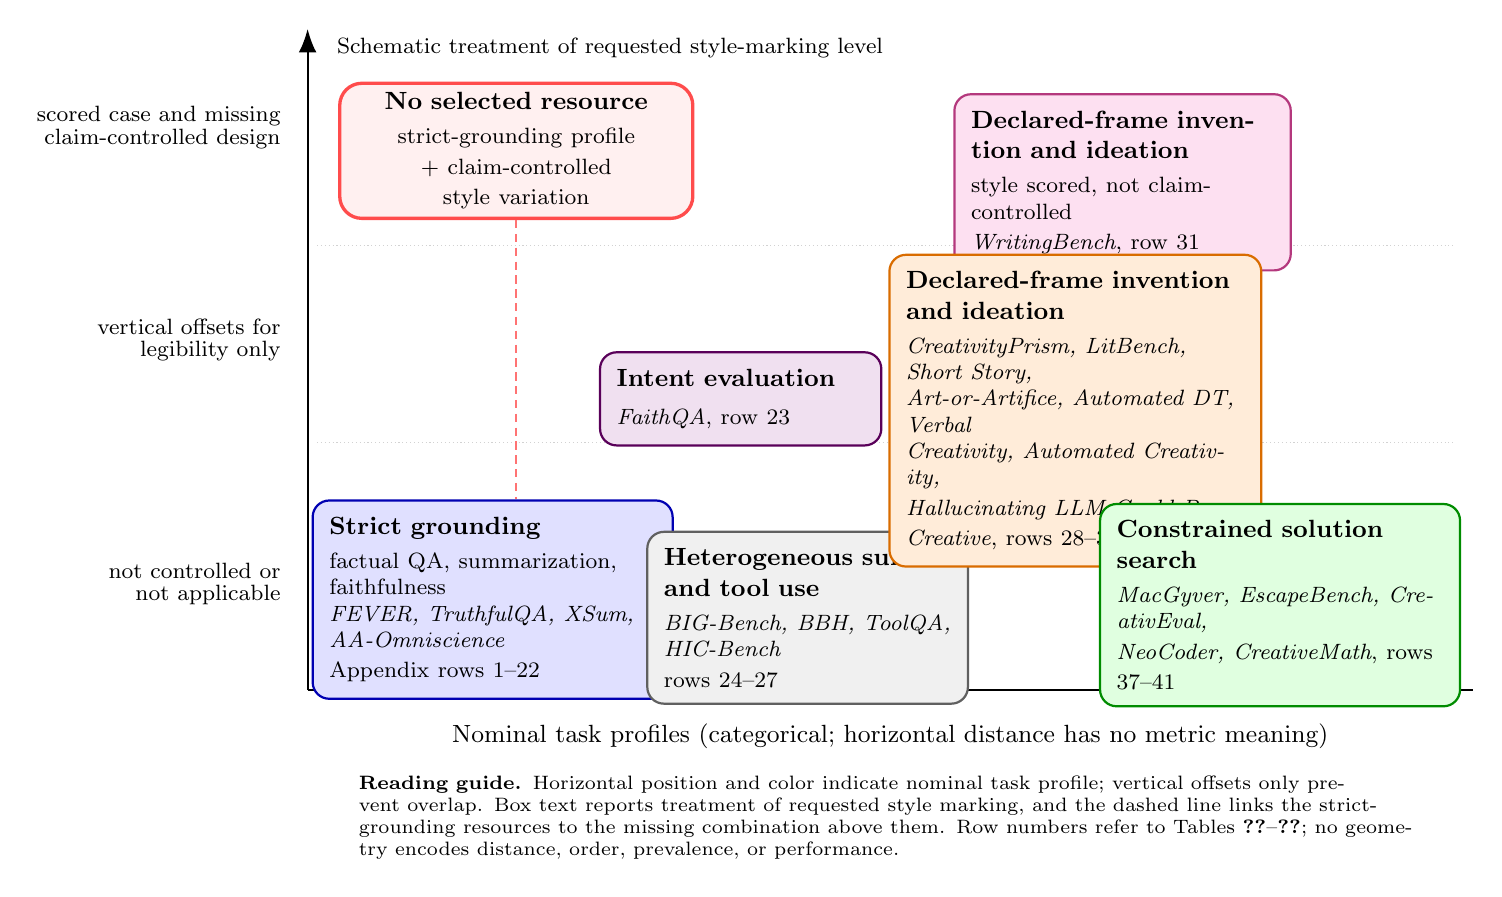
\begin{tikzpicture}[
    x=1cm,y=1cm,
    >=Latex,
    font=\small,
    axis/.style={thick,-{Latex[length=3mm]}},
    clusterbox/.style={
        rounded corners=6pt,
        thick,
        align=left,
        inner sep=6pt,
        text width=3.55cm
    },
    note/.style={font=\scriptsize,align=left}
]

% Schematic axes: vertical offsets are retained only for legibility.
% Horizontal grouping only: no direction and no metric interpretation.
\draw[thick] (0,0) -- (14.8,0);
\node[below,align=center] at (7.4,-0.30)
  {Nominal task profiles
   (categorical; horizontal distance has no metric meaning)};
\draw[axis] (0,0) -- (0,8.4);
\node[anchor=west,font=\footnotesize] at (0.25,8.15)
  {Schematic treatment of requested style-marking level};

\node[left,align=right] at (-0.22,1.35)
  {\footnotesize not controlled or\\[-1mm]\footnotesize not applicable};
\node[left,align=right] at (-0.22,4.45)
  {\footnotesize vertical offsets for\\[-1mm]\footnotesize legibility only};
\node[left,align=right] at (-0.22,7.15)
  {\footnotesize scored case and missing\\[-1mm]\footnotesize claim-controlled design};
\draw[densely dotted,gray!35] (0.12,3.15) -- (14.55,3.15);
\draw[densely dotted,gray!35] (0.12,5.65) -- (14.55,5.65);

% Missing combination targeted by the proposed benchmark.
\node[
  draw=red!70,very thick,rounded corners=8pt,fill=red!6,
  text width=4.25cm,minimum height=1.65cm,align=center
] (gap) at (2.65,6.85)
  {\textbf{No selected resource}\\[1mm]
   \footnotesize strict-grounding profile\\
   \footnotesize + claim-controlled style variation};

% The only selected protocol that explicitly scores a requested style
% constraint, without holding canonical claim content fixed.
\node[clusterbox,draw=magenta!70!black,fill=magenta!12,
  text width=3.85cm] (writing) at (10.35,6.45) {
  {\bfseries Declared-frame invention and ideation}\\[1mm]
  \footnotesize style scored, not claim-controlled\\
  \footnotesize \textit{WritingBench}, row 31
};

% Resources whose requested style-marking level is not controlled.
\node[clusterbox,draw=blue!70!black,fill=blue!12,
  text width=4.15cm] (strict) at (2.35,1.15) {
  {\bfseries Strict grounding}\\[1mm]
  \footnotesize factual QA, summarization, faithfulness\\
  \footnotesize \textit{FEVER, TruthfulQA, XSum, AA-Omniscience}\\
  \footnotesize Appendix rows 1--22
};

\node[clusterbox,draw=violet!70!black,fill=violet!12,
  text width=3.15cm] (intent) at (5.50,3.70) {
  {\bfseries Intent evaluation}\\[1mm]
  \footnotesize \textit{FaithQA}, row 23
};

\node[clusterbox,draw=gray!75!black,fill=gray!12,
  text width=3.65cm] (mixed) at (6.35,0.92) {
  {\bfseries Heterogeneous suites and tool use}\\[1mm]
  \footnotesize \textit{BIG-Bench, BBH, ToolQA, HIC-Bench}\\
  \footnotesize rows 24--27
};

\node[clusterbox,draw=orange!85!black,fill=orange!15,
  text width=4.30cm] (creative) at (9.75,3.55) {
  {\bfseries Declared-frame invention and ideation}\\[1mm]
  \footnotesize \textit{CreativityPrism, LitBench, Short Story,}\\
  \footnotesize \textit{Art-or-Artifice, Automated DT, Verbal}\\
  \footnotesize \textit{Creativity, Automated Creativity,}\\
  \footnotesize \textit{Hallucinating LLM Could Be Creative}, rows 28--30, 32--36
};

\node[clusterbox,draw=green!55!black,fill=green!12,
  text width=4.15cm] (solution) at (12.35,1.08) {
  {\bfseries Constrained solution search}\\[1mm]
  \footnotesize \textit{MacGyver, EscapeBench, CreativEval,}\\
  \footnotesize \textit{NeoCoder, CreativeMath}, rows 37--41
};

% Vertical link: the empty region sits directly above the strict grounding
% cluster, in the same profile column.
\draw[densely dashed,red!55,line width=0.7pt]
  (gap.south) -- (gap.south |- strict.north);

\node[note,text width=13.5cm] at (7.40,-1.62) {
\textbf{Reading guide.}
Horizontal position and color indicate nominal task profile; vertical offsets
only prevent overlap. Box text reports treatment of requested style marking,
and the dashed line links the strict-grounding resources to the missing
combination above them. Row numbers refer to
Tables~\ref{tab:full-mapping-factual-a}--\ref{tab:full-mapping-creative}; no
geometry encodes distance, order, prevalence, or performance.
};
\end{tikzpicture}%
}

\caption{\textbf{Selected resources by nominal task profile and treatment of
requested style-marking level.}
WritingBench is the only selected resource that scores requested style, but it
does not hold canonical claim content fixed. The remaining resources do not
control requested style in a claim-preserving comparison. The empty top-left
region marks this missing combination for strict grounding. The coding in
Appendix~\ref{app:mapping}, rather than the figure geometry, supports the
broader result that no selected resource represents all three truth-contract
fields while controlling claim-preserving style variation.}
\label{fig:profiles}
\end{figure}
\FloatBarrier

\section{Worked Cases}\label{sec:cases}

The five cases state the rule's consequences under explicit conditions.
They are constructed comparisons, not sampled model outputs or experimental
results. Each identifies what remains fixed, what changes, and the predicted
outcome. Case~B changes several factors; Case~E requires independently
confirmed claim equivalence before it can test evaluator robustness.
Figure~\ref{fig:case-transitions} provides a compact guide.

\begin{figure}[!ht]
\centering
\resizebox{\textwidth}{!}{%
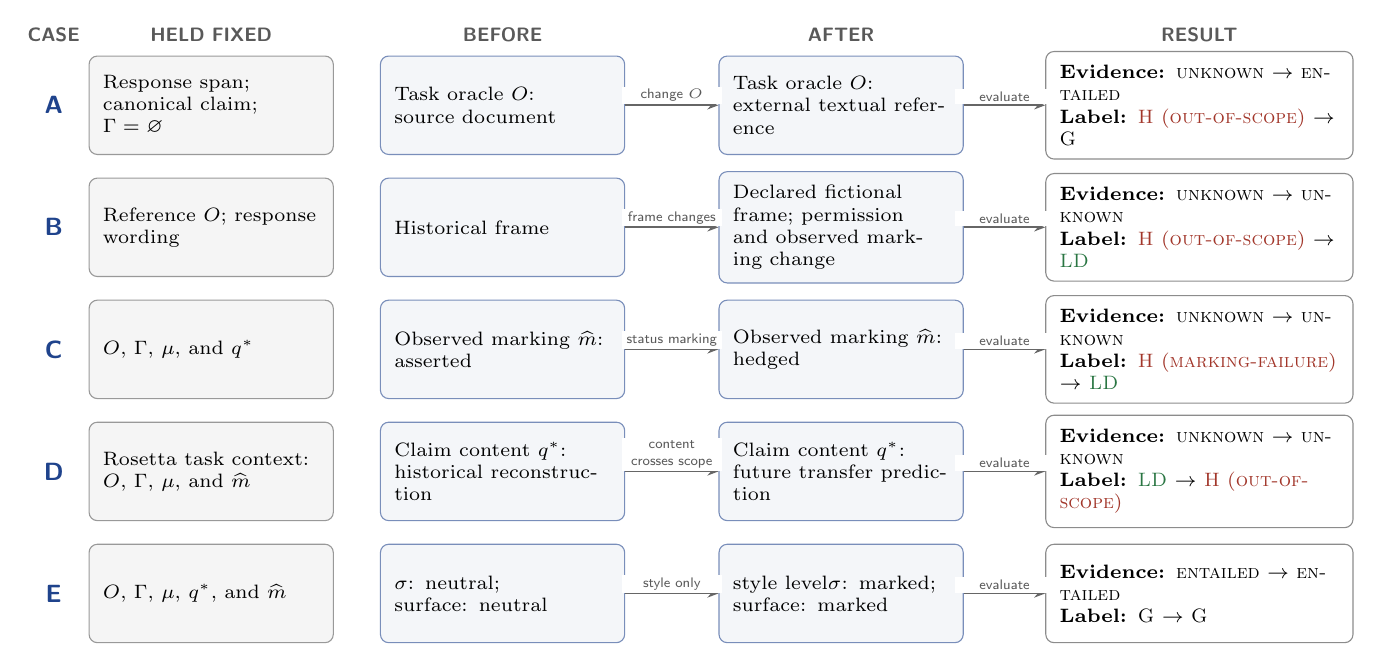
\begin{tikzpicture}[x=1cm,y=1cm,font=\small,
  every node/.style={inner sep=0pt}]
  \definecolor{caseblue}{RGB}{31,67,140}
  \definecolor{casegreen}{RGB}{42,118,67}
  \definecolor{casered}{RGB}{162,54,42}
  \tikzset{
    colhead/.style={font=\scriptsize\sffamily\bfseries,text=black!65,
      align=center},
    caselabel/.style={font=\small\sffamily\bfseries,text=caseblue,
      align=center},
    fixed/.style={rectangle,rounded corners=3pt,draw=black!40,fill=gray!8,
      text width=2.75cm,minimum height=1.25cm,align=left,
      font=\scriptsize,inner sep=5pt},
    condition/.style={rectangle,rounded corners=3pt,draw=caseblue!60,
      fill=caseblue!5,text width=2.75cm,minimum height=1.25cm,
      align=left,font=\scriptsize,inner sep=5pt},
    outcome/.style={rectangle,rounded corners=3pt,draw=black!45,fill=white,
      text width=3.55cm,minimum height=1.25cm,align=left,
      font=\scriptsize,inner sep=5pt},
    transition/.style={-{Stealth[length=4pt,width=3pt]},semithick,
      draw=black!60},
    transitionlabel/.style={font=\tiny\sffamily,text=black!65,
      align=center,text width=1.20cm,fill=white,inner sep=1pt},
    beforeafter/.style={font=\tiny\sffamily\bfseries,text=black!55,
      align=center}
  }

  \node[colhead] at (0,0.90) {CASE};
  \node[colhead] at (2.00,0.90) {HELD FIXED};
  \node[colhead] at (5.70,0.90) {BEFORE};
  \node[colhead] at (10.00,0.90) {AFTER};
  \node[colhead] at (14.55,0.90) {RESULT};

  % Case A
  \node[caselabel] at (0,0) {A};
  \node[fixed] (a-fixed) at (2.00,0)
    {Response span; canonical claim; $\Gamma=\varnothing$};
  \node[condition] (a-before) at (5.70,0)
    {Task oracle $O$:\\source document};
  \node[condition] (a-after) at (10.00,0)
    {Task oracle $O$:\\external textual reference};
  \draw[transition] (a-before.east) --
    node[transitionlabel,above] {change $O$} (a-after.west);
  \node[outcome] (a-result) at (14.55,0)
    {\textbf{Evidence:} \textsc{unknown} $\to$ \textsc{entailed}\\
     \textbf{Label:} \textcolor{casered}{\Hall{} (\textsc{out-of-scope})}
     $\to$ \Grd};
  \draw[transition] (a-after.east) --
    node[transitionlabel,above] {evaluate} (a-result.west);

  % Case B
  \node[caselabel] at (0,-1.55) {B};
  \node[fixed] (b-fixed) at (2.00,-1.55)
    {Reference $O$; response wording};
  \node[condition] (b-before) at (5.70,-1.55)
    {Historical frame};
  \node[condition] (b-after) at (10.00,-1.55)
    {Declared fictional frame; permission and observed marking change};
  \draw[transition] (b-before.east) --
    node[transitionlabel,above] {frame changes} (b-after.west);
  \node[outcome] (b-result) at (14.55,-1.55)
    {\textbf{Evidence:} \textsc{unknown} $\to$ \textsc{unknown}\\
     \textbf{Label:} \textcolor{casered}{\Hall{} (\textsc{out-of-scope})}
     $\to$ \textcolor{casegreen}{\LD}};
  \draw[transition] (b-after.east) --
    node[transitionlabel,above] {evaluate} (b-result.west);

  % Case C
  \node[caselabel] at (0,-3.10) {C};
  \node[fixed] (c-fixed) at (2.00,-3.10)
    {$O$, $\Gamma$, $\mu$, and $q^*$};
  \node[condition] (c-before) at (5.70,-3.10)
    {Observed marking $\widehat{m}$:\\asserted};
  \node[condition] (c-after) at (10.00,-3.10)
    {Observed marking $\widehat{m}$:\\hedged};
  \draw[transition] (c-before.east) --
    node[transitionlabel,above] {status marking} (c-after.west);
  \node[outcome] (c-result) at (14.55,-3.10)
    {\textbf{Evidence:} \textsc{unknown} $\to$ \textsc{unknown}\\
     \textbf{Label:} \textcolor{casered}{\Hall{} (\textsc{marking-failure})}
     $\to$ \textcolor{casegreen}{\LD}};
  \draw[transition] (c-after.east) --
    node[transitionlabel,above] {evaluate} (c-result.west);

  % Case D
  \node[caselabel] at (0,-4.65) {D};
  \node[fixed] (d-fixed) at (2.00,-4.65)
    {Rosetta task context:\\$O$, $\Gamma$, $\mu$, and $\widehat{m}$};
  \node[condition] (d-before) at (5.70,-4.65)
    {Claim content $q^*$:\\historical reconstruction};
  \node[condition] (d-after) at (10.00,-4.65)
    {Claim content $q^*$:\\future transfer prediction};
  \draw[transition] (d-before.east) --
    node[transitionlabel,above] {content crosses scope} (d-after.west);
  \node[outcome] (d-result) at (14.55,-4.65)
    {\textbf{Evidence:} \textsc{unknown} $\to$ \textsc{unknown}\\
     \textbf{Label:} \textcolor{casegreen}{\LD} $\to$
     \textcolor{casered}{\Hall{} (\textsc{out-of-scope})}};
  \draw[transition] (d-after.east) --
    node[transitionlabel,above] {evaluate} (d-result.west);

  % Case E
  \node[caselabel] at (0,-6.20) {E};
  \node[fixed] (e-fixed) at (2.00,-6.20)
    {$O$, $\Gamma$, $\mu$, $q^*$, and $\widehat{m}$};
  \node[condition] (e-before) at (5.70,-6.20)
    {$\sigma$: neutral;\\surface: neutral};
  \node[condition] (e-after) at (10.00,-6.20)
    {style level$\sigma$: marked;\\surface: marked};
  \draw[transition] (e-before.east) --
    node[transitionlabel,above] {style only} (e-after.west);
  \node[outcome] (e-result) at (14.55,-6.20)
    {\textbf{Evidence:} \textsc{entailed} $\to$ \textsc{entailed}\\
     \textbf{Label:} \Grd{} $\to$ \Grd{}};
  \draw[transition] (e-after.east) --
    node[transitionlabel,above] {evaluate} (e-result.west);
\end{tikzpicture}%
}
\caption{\textbf{Five worked cases as a transition diagram.}
Each row keeps the fields listed as fixed in the corresponding case, shows the
before-to-after change with a directional arrow, and then shows the resulting
evidence-state and claim-label transitions. Case~B is explicitly
multifactorial. Case~E changes the requested style and its realization together; the other contrasts retain the quantities listed as fixed. The diagram renders the
constructed tests developed below and does not add an empirical comparison.}
\label{fig:case-transitions}
\end{figure}
\FloatBarrier
\paragraph{Case A: changing the task oracle}
In XSum, a summary statement may be absent from the source document while
remaining correct against external evidence \citep{maynez_faithfulness_2020}.
\textbf{Purpose.} To test that the claim label depends on which oracle the task
designates, not on the claim alone.
\par\textbf{Fixed.} The response span, canonical claim, and empty permission scope.
\par\textbf{Changed.} One condition uses the source document as the task oracle;
the other design uses a fixed collection of external textual evidence.
Each reference remains fixed within its own design.
\par\textbf{Predicted result.} Relative to the source document, the claim is
\textsc{unknown}. Because $\Gamma=\varnothing$, it receives the hallucination
label with reason code \textsc{out-of-scope}. Relative to the external task
oracle, the same claim is \textsc{entailed} and receives the grounded label.

\paragraph{Case B (multi-factor): a contextualization boundary across historical
and fictional frames}
This case changes permission and observed framing together; it is not a
single-factor test of permission.
\textbf{Purpose.} To distinguish a historical assertion from content offered
inside a declared fiction without changing the reference.
\par\textbf{Fixed.} The bounded Rosetta Stone reference and the constructed
string ``The complete stele stood near a temple entrance.''
\par\textbf{Changed.} The historical condition asks for a strictly grounded
museum label. The fictional condition permits an invented setting and places
the same sentence inside a declared alternate-history story. Permission and
observed status marking change; the reference does not.
\par\textbf{Predicted result.} The placement remains \textsc{unknown} relative
to the fixed reference. In the historical condition, $\Gamma=\varnothing$, so
it receives the hallucination label with reason code \textsc{out-of-scope}.
In the fictional condition, the task permits the placement and the declared
frame supplies the required marking, so it receives licensed divergence.
The canonical record retains the fictional status; unchanged wording does not
by itself establish an unchanged commitment.

\paragraph{Case C: changing the observed status marking}
This controlled contrast reuses the Rosetta Stone reconstruction from
Section~\ref{subsec:contract}. The permission scope allows one plausible
placement, and the required status marking requires it to be presented as
conjecture.
\textbf{Purpose.} To test that permission alone is not enough: presentation is
part of the contract.
\par\textbf{Fixed.} The task oracle $O$, $\Gamma$, $\mu$, the content $q^*$
that the complete stele stood near a temple entrance, and its \textsc{unknown}
evidence state.
\par\textbf{Changed.} Only the observed status marking $\widehat{m}$.
\par\textbf{Predicted result.} ``The complete stele stood near a temple
entrance'' receives the hallucination label with reason code
\textsc{marking-failure}. ``One possible reconstruction places the complete
stele near a temple entrance'' receives the licensed-divergence label. The
content, evidence state, and all three contract fields are identical; only the
wording that signals epistemic status differs.

\paragraph{Case D: testing a scope boundary}
This case returns to the Rosetta Stone museum-label task, whose permission scope
allows one marked historical reconstruction.
\textbf{Purpose.} To test that a permission scope has a boundary, and that the
boundary is drawn around content rather than around the frame.
\par\textbf{Fixed.} The task oracle $O$, $\Gamma$, $\mu$, the \textsc{unknown}
evidence state, and conjectural observed marking $\widehat{m}$.
\par\textbf{Changed.} Only the content $q^*$: ``One possible reconstruction
places the complete stele near a temple entrance'' versus the constructed
prediction ``One possibility is that the stone will be returned to Egypt next
year.''
\par\textbf{Predicted result.} The historical reconstruction lies inside
$\Gamma$ and receives the licensed-divergence label. The future transfer
prediction is also \textsc{unknown} and marked as a possibility, but it is not
the historical reconstruction that the task permits. It falls outside
$\Gamma$ and receives the hallucination label with reason code
\textsc{out-of-scope}.

\paragraph{Case E: changing surface realization with a fixed claim}
This case isolates a change in stylistic realization while holding both
truth-conditional content and epistemic status fixed.
\textbf{Purpose.} To test whether claim-preserving stylistic variation leaves
the claim label unchanged.
\par\textbf{Fixed.} The task oracle $O$ of the Rosetta Stone example of
Figure~\ref{fig:claim-label-annotation}, $\Gamma$, $\mu$, the content component
$q^*$ that the decree appears in hieroglyphic, Demotic, and Greek, and the
observed status marking $\widehat{m}$.
\par\textbf{Changed.} Only requested style-marking level $\sigma$ and surface
realization; the two responses are designed as a claim-preserving style
variation.
Neutral realization: ``The decree is written in hieroglyphic, Demotic, and
Greek.''
Marked realization: ``The same message speaks three times over: once in
hieroglyphs, once in Demotic, once in Greek.''
\par\textbf{Predicted result.} Both variants recover the same canonical claim
and receive the grounded label when the task oracle entails it. The observed
style-marking level and the style-marking alignment result are reported
separately.
After independent adjudication confirms equivalence, a difference in recovered claims or labels would identify an evaluator failure on this test.
It would not, by itself, establish that style generally changes claim recovery.

Together, the cases examine changes in the task oracle, discourse frame,
observed status marking, claim content relative to a fixed permission scope, and surface realization. Their
predicted transitions and invariances become the annotation and benchmark
hypotheses in the research agenda: the first studies test whether the relevant
fields can be recovered reliably, then whether controlled changes produce the
labels predicted here.


\section{Research Agenda}\label{sec:agenda}

The agenda distinguishes three questions: can the framework be applied
reliably, does explicit representation help evaluation, and how far does it
generalize? Table~\ref{tab:agenda} retains seven priorities. The first three
establish measurement, the next two assess practical use, and the last two
examine broader settings and extensions.

Comparisons should include a combined factuality and instruction-following
baseline. When testing the decision rule, methods should share the oracle and
claim-recovery inputs. Recovery studies should instead vary that component
explicitly. Independent annotations should record evidence, permission,
marking, and acceptability without defining every gold judgment solely by
our rule. Otherwise, agreement tests only implementation, not the usefulness
or acceptability of the convention. Thresholds and comparison criteria should
be declared in advance.

\begin{table}[!ht]
\centering
\small
\setlength{\tabcolsep}{5pt}
\renewcommand{\arraystretch}{1.10}
\caption{\textbf{The research agenda in one view.} The table lists seven
priorities and their open questions. The corresponding paragraphs give the
study designs, measures, and critical comparisons.}
\label{tab:agenda}
\begin{tabularx}{\linewidth}{@{}P{0.24\linewidth}Y@{}}
\toprule
\textbf{Priority} & \textbf{Open question}\\
\midrule
1.~Contract annotation
& Can evaluators consistently identify the task oracle $O$, permission scope
$\Gamma$, and required status marking $\mu$ from a task context?\\\addlinespace[2pt]
2.~Factorial benchmark
& Do claim labels change as predicted when one contract field changes and the rest are held fixed?\\\addlinespace[2pt]
3.~Style-robust recovery
& Does claim recovery return the same claims across matched realizations of one claim?\\\addlinespace[2pt]
4.~Response-level record
& What must be added to a claim trace to judge a complete response?\\\addlinespace[2pt]
5.~Mitigation
& Can hallucination be reduced without suppressing permitted divergence?\\\addlinespace[2pt]
6.~Generalization
& Do the contract fields remain applicable across other domains, genres, and
languages?\\\addlinespace[2pt]
7.~Temporal and agentic
& How does a contract update over time, and how does a claim-level failure
propagate into an action?\\
\bottomrule
\end{tabularx}
\end{table}
\FloatBarrier

\paragraph{1. Contract annotation}
A public codebook should specify oracle sources and authority, permission
boundaries, marking requirements, and claim interpretation. Pilot studies
should annotate each field separately, record genuine disagreement, and measure
agreement, adjudication rate, annotation time, and error sources. Contract
annotations may be reused across responses to the same task; claims still
require response-specific recovery.
\emph{Critical test.} Persistent field-level disagreement challenges the
operational definitions. High cost without diagnostic benefit weakens the
practical case for explicit annotation.

\paragraph{2. Controlled contrasts}
A factorial benchmark should vary $\Gamma$ or $\mu$ while holding the
textual oracle fixed. Comparisons of $O$ require separate evaluation designs
with their own fixed references. Include a contradicted claim under matched
tasks that respectively permit and forbid that specific contradiction. Changing required marking $\mu$
is different from changing observed marking $\widehat{m}$, as Case~C does; protocols
must state which is manipulated. Frame changes such as Case~B require separate
analysis because they can also change the contextualized claim.
Studies should measure evidence-state agreement, claim labels, reason codes,
and independent judgments of task acceptability.
\emph{Critical test.} A change in intended commitment invalidates a purported
single-factor contrast. Systematic rejection of LD for explicitly permitted and adequately marked
contradictions challenges this extension of the evaluation convention. An equally accurate and informative baseline
limits the benefit of a separate implementation, not the need to consider
permission.

\paragraph{3. Style-robust recovery and error localization}
Matched realizations should preserve $q^*$ and $\widehat{m}$ under a fixed contract
while varying style. Independent adjudication must establish those matches.
Studies should measure omissions, spurious claims, under-decomposition,
over-decomposition, altered status, and downstream label errors.
Evaluation with and without access to requested style can test whether that
context helps recovery while response text remains fixed. The trace should
identify whether a disputed label arose during recovery, verification, or a
contract check.
\emph{Critical test.} Instability on validated pairs challenges evaluator
robustness. No useful improvement in error localization limits the diagnostic
benefit of the additional trace.

\paragraph{4. Response-level evaluation}
Studies should compare the content verdict with independent assessments of
reasoning, consistency, completeness, relevance, and task success. They should
also examine coverage thresholds and constraints such as reconstruction quotas.
Alternative aggregations require sensitivity analysis: conclusions and model
rankings may depend on the chosen policy. Style alignment and creativity remain
separate reported outcomes.
\emph{Critical test.} If additional components provide no information beyond
the trace in a given setting, their practical value there is limited. This
does not establish that local labels logically guarantee global correctness.

\paragraph{5. Mitigation without suppressing permitted divergence}
A lower hallucination score may result from suppressing unknown content,
including content the task requested or allowed. Compare retrieval,
verification, abstention, and constrained generation on H reduction, retention
of grounded and licensed content, style alignment, and creative-task success.
Report outcomes by contract, with uncertainty for human creative judgments,
and expose trade-offs rather than hiding them in one scalar.
\emph{Critical test.} A method that improves only by removing permitted
content has not established a benefit for tasks requiring such content. This
challenges the mitigation claim, not the distinction between H and LD.

\paragraph{6. Generalization}
Replicate annotation and contrast studies across domains, genres, and languages.
Report field-level agreement and costs separately, because failure to identify
permission differs from failure to interpret a hedge. The provisional style
scale also needs validation beyond the museum examples.
\emph{Critical test.} Systematic disagreement tied to a domain or language
limits the generality of the relevant definition or procedure.

\paragraph{7. Temporal updates and agentic action}
Multi-step tasks may change the available evidence and consume earlier claims
in later actions. Extending the present fixed-reference framework would require time-indexed
contracts. Future work should record
why an oracle or permission changed, and trace claim-level failures into
subsequent actions. Updates must follow the task protocol rather than justify
an observed output after the fact.
\emph{Critical test.} If a static evaluation performs equally well on the
chosen action-level outcomes, the proposed temporal extension adds no measured
benefit in that setting.

\section{Discussion}\label{sec:discussion}

\subsection{What Is Relative and What Is Not}\label{subsec:relative}

Our position concerns the conditions for assigning an evaluation label.
A task can authorize a possibility without making it true. Likewise,
changing the designated oracle changes the evidence relation used for
evaluation, not the underlying world's facts. The proposed H convention covers
unknown or contradicted departures that are unauthorized or inadequately
marked. An authorized contradiction remains a contradiction even when labeled LD.
Its terminology therefore needs empirical scrutiny, especially for an openly
hedged but out-of-scope proposal. Retaining evidence states and reason codes
keeps these cases distinguishable even when a reader disputes the umbrella term.

Theoretical results on hallucination provide context for reliability concerns,
not a proof of this particular contract. Prior work gives lower bounds under
calibration assumptions or discusses limits grounded in computability
\citep{kalai_calibrated_2024,xu_hallucination_2024,banerjee_llms_2024}.
Their assumptions differ; they do not determine a constant deployment error
rate or exclude negligible rates in a specified setting
\citep{suzuki_negligible_2025}. The bounded-oracle argument in this paper does
not depend on proving that hallucination is unavoidable.

The manuscript's AA-Omniscience snapshot supplies a separate descriptive
illustration \citep{jackson_aaomniscience_2025,artificialanalysis_omniscience_leaderboard_2026}.
Appendix~\ref{app:omniscience} preserves its date, metric definitions, and
limitations. Comparisons across heterogeneous model configurations do not
identify a causal scaling law. They also do not establish that truth-contract
annotation improves evaluation. That question belongs to the agenda above.

\subsection{Interpreting the Response-Level Record}

The record in Section~\ref{subsec:response} makes different conclusions visible.
A compliant content verdict concerns the evaluated claims under a coverage
policy; it does not imply factual truth, creative success, or satisfaction of
every response-level requirement. An indeterminate verdict records an
incomplete evaluation, not necessarily a model error. Benchmarks should retain
that outcome rather than silently discard it.

These distinctions matter for mitigation. A claim trace can reveal whether a
method reduced contradictions, removed unauthorized additions, or improved
marking. Creative-task assessment then asks whether useful permitted content
was preserved. A severity-weighted score may support triage, but it cannot
erase an observed violation or change a claim's label after assessment.

\subsection{Limitations and Open Decisions}

The framework specifies a local evaluation convention, not a validated
evaluator. Its application depends on recoverable commitments, an explicit
contract, and reliable oracle adjudication. Separating $q^*$ from $\widehat{m}$ is
particularly delicate when modality or fictional framing changes meaning.
Unresolved cases require an explicit failure record, not forced labels.

The response-level verdict has limited scope. It does not verify inference
validity, cross-claim consistency, omissions, relevance, or quotas. The
reconstruction example makes the quota limitation concrete: local eligibility
alone cannot enforce a maximum number of additions. Further response-level
rules require specification and validation without silently redefining G/H/LD.

The descriptive evidence also has limits. The sample is purposive, its
selection procedure remains incompletely documented, and its coding needs
independent verification. The oracle interpretation for constrained-solution
resources is an identified unresolved issue. The style scale is provisional,
and constructed cases do not establish annotation reliability or evaluator
robustness. These limits distinguish the present conceptual contribution from
the evidence needed to support practical deployment.

\section{Conclusion}\label{sec:conclusion}

We argue that hallucination evaluation needs an explicit truth contract.
Evidence establishes what is supported; task conditions determine whether
unknown or contradicted content may be introduced and how it must be presented. Making those
roles explicit allows permitted divergence to remain distinguishable from
contract violations without treating creative value as evidence of truth.

The paper specifies a claim-level rule and a response-level record, examines
forty-one resources through a descriptive coding, and develops five constructed
cases. The resulting agenda separates annotation reliability, robustness, and
practical benefit. The next step is to test these properties against comparably
informed evaluation procedures. The goal is reliable grounding where required,
transparent divergence where permitted, and separate assessment of the
response's creative and other task-specific qualities.
\clearpage

\appendix

\appendixsection{Response-Level Record, Procedural Failures, and Optional Aggregation}%
\phantomsection
\makeatletter\def\@currentlabel{A}\makeatother\label{app:diagnostics}

Section~\ref{sec:framework} defines the truth contract, claim recovery,
canonicalization, claim verification, the claim-labeling rule, and the
style-marking alignment check.
Those definitions govern decisions about individual claims. This appendix
specifies what an evaluation publishes after those decisions. It defines the
response-level record, the procedural failures that can prevent labeling, the
stability test for claim recovery under claim-preserving style variation, and
the role of optional aggregation.


\paragraph{Reporting and aggregation details}
Section~\ref{subsec:response} defines the ordered content verdict and recovery
coverage. Publish that verdict with its coverage threshold, the claim trace,
and any procedural failures. A reliably adjudicated H takes precedence over
failures affecting other claims.

Style-marking alignment is \textsc{match}, \textsc{mismatch}, or
\textsc{not applicable} when the task specifies no target. Compare the requested
level with the independently assessed observed level using the provisional
three-level scale in Section~\ref{subsec:style}. Withhold this component when
either level cannot be adjudicated; do not convert uncertainty into a mismatch.
The categorical comparison may later be replaced by a validated tolerance or
ordinal distance rule.

Creative-task success is \textsc{pass}, \textsc{fail}, \textsc{not assessed},
or a task-specific score under an explicit rubric. Report the criteria and
unit of analysis. Novelty, usefulness, quality, and diversity should not be
silently substituted for one another.

Optional proportional, severity-weighted, or task-specific aggregations may
support ranking. Declare the policy before evaluation, retain every underlying
label, and report sensitivity to plausible alternatives. Such scores do not
override the default record of an observed violation. Global logical validity,
consistency, completeness, relevance, and quotas remain separate diagnostics.

\paragraph{Procedural failures}

A \emph{procedural failure} is a breakdown in the evaluation procedure itself
rather than in the response.
It is recorded in place of a claim label, and the affected span is left
unlabeled; it never receives \Grd, \Hall, or \LD.
Three conditions must hold before any claim label can be assigned: the
evaluator must obtain a stable canonical claim, the task context must determine
the three contract fields, and claim verification must resolve the claim to one
evidence state.
Each condition can fail in a distinct way.

\paragraph{Failures of claim recovery}
The evaluator may be unable to obtain a stable canonical claim.
Span-selection, claim recovery, canonicalization, and matching errors all have
this effect.
They may cause an evaluator to omit a recoverable claim, create a spurious
canonical claim, under-decompose distinct commitments into one claim,
over-decompose one commitment into several claims, or alter $q^*$ or $\widehat{m}$.
If no stable canonical claim can be obtained, no claim label is assigned to the
affected span.

\paragraph{Failures of the truth contract or task oracle}
The evaluator may instead be unable to apply the contract to a claim it has
recovered. Four failures have this effect.
\begin{description}
  \item[Truth-contract specification failure.] The task context does not
        determine $O$, $\Gamma$, and $\mu$.
  \item[Task-oracle specification failure.] $O$ does not identify admissible
        sources, temporal scope, authority relations, or a conflict-resolution
        procedure precisely enough for the task.
  \item[Task-oracle adequacy failure.] Required sources are missing or inaccessible, the source version violates the protocol, or an unresolved conflict prevents the designated procedure from applying. Silence in a correctly specified bounded oracle is not this failure.
  \item[Adjudication failure.] The evaluator cannot resolve the task oracle
        into a single evidence state.
\end{description}
In each case the evaluator records the failure and leaves the affected span
unlabeled.
Silence is not one of these failures: a correctly instantiated bounded task
oracle that does not entail or contradict a claim yields the
\textsc{unknown} evidence state, which the contract is designed to handle.
A blocking procedural failure prevents a compliant verdict and does not create an automatic \textsc{unknown} evidence state. If another claim reliably receives H, the ordered rule still returns \textsc{contract-violating}; otherwise it returns \textsc{indeterminate}.
Recent fact-verification work shows that these outcomes are easy to conflate in
practice. How an \textsc{unknown} evidence condition is constructed shapes what
a verifier learns and can hide genuine adjudication difficulty
\citep{qiu_evidence_2026}. Separately, a single global faithfulness label can
mask sentence-level adjudication disagreement through an averaging bias
\citep{zhang_averaging_2026}.

\paragraph{An example}
Suppose two annotators read the closing span of a museum panel, ``the winter
that would not lift''.
One recovers a claim about the severity of that winter; the other recovers no
truth-conditional claim at all.
The two annotators disagree about which claim the span commits to, not about
which label a shared claim deserves.
The evaluation therefore records a claim-recovery failure for that span instead
of a label disagreement.

A response that does not realize the requested style-marking level is not a
procedural failure.
That mismatch is recorded through style-marking alignment, whereas a canonical
claim that violates the truth contract is handled by the claim-labeling rule.


\paragraph{Claim-preserving style variation test}
Consider three expert-adjudicated responses $y_0,y_1,y_2$ produced under task
contexts that differ only in requested style-marking level, with
$\sigma_{p_0}=0$, $\sigma_{p_1}=1$, and $\sigma_{p_2}=2$.
The test asks two questions: do the responses yield the same canonical claims,
and do those matched claims receive the same labels? After one-to-one
adjudicated matching, let $\mathcal C^*(y_i,p_i)$ denote each set of canonical
claims $c^*=(q^*,\widehat{m})$. Claim-preserving style variation requires the
matched-claim-set condition
$\mathcal C^*(y_0,p_0)=\mathcal C^*(y_1,p_1)=\mathcal C^*(y_2,p_2)$.
Thus, matched claims retain the same $q^*$ and $\widehat{m}$ components, although their
surface strings and observed style-marking levels may differ. With $O$,
$\Gamma$, and $\mu$ fixed, every matched canonical claim $c_j^*$ must also
receive the same claim label (\Grd, \Hall, or \LD) under $y_0,p_0$, $y_1,p_1$,
and $y_2,p_2$.

\begin{itemize}
  \item \emph{Claim recovery error}: a recoverable claim is dropped or a
        spurious claim is added during claim recovery.
  \item \emph{Canonicalization error}: canonicalization alters $q^*$ or
        $\widehat{m}$.
  \item \emph{Claim-label instability}: matched canonical claims receive
        different labels when $O$, $\Gamma$, and $\mu$ are fixed.
  \item \emph{Style-marking alignment error}: the evaluator
        incorrectly classifies the match between requested and observed
        style-marking levels.
  \item \emph{Optional-aggregation sensitivity}: a response comparison
        changes when the evaluator changes an optional rule applied to the
        claim-level labels and diagnostics.
\end{itemize}

Claim recovery and claim-label diagnostics require expert-adjudicated canonical
claim matches.
Style-marking alignment errors require an independently
adjudicated comparison between requested and observed style-marking levels.
Claim-label instability is an error only when $O$, $\Gamma$, and $\mu$ remain fixed.
When $\Gamma$ or $\mu$ changes, the same departure may
intentionally change from the hallucination label to the licensed-divergence
label; its evidence state remains unchanged.

Optional scalar aggregation may support ranking, but it does not replace the
response-level record or its component diagnostics. Comparisons should report
sensitivity to plausible aggregation rules rather than present one rule as
uniquely determined.

\appendixsection{Resource Mapping}%
\phantomsection
\makeatletter\def\@currentlabel{B}\makeatother\label{app:mapping}
\renewcommand*{\theHtable}{B.\arabic{table}}

Tables~\ref{tab:full-mapping-factual-a}--\ref{tab:full-mapping-creative} list the forty-one resources used in the purposive mapping.
Each row reports a task-oracle type and its task-specific instantiation, a
separate quality or task-success criterion, treatment of requested
style-marking level, permission scope $\Gamma$, and required status marking
$\mu$ under the nominal task profiles used in Figure~\ref{fig:profiles}.

\paragraph{Coding vocabulary}
Each coded field uses one value from the following list. Parenthetical text may
retain a task-specific qualifier, but it does not create an additional code.

\begin{description}
  \item[Nominal task profile.]
  \emph{strict grounding};
  \emph{intent evaluation};
  \emph{declared-frame invention and ideation};
  \emph{constrained solution search};
  \emph{heterogeneous suites and tool use}.

  \item[Adjudication standard (inherited column $O$).]
  This descriptive vocabulary includes nontextual standards outside the present
  framework. The column is preserved for traceability, not as an expanded
  definition of our fixed textual oracle.
  \emph{source document}, a supplied document treated as authoritative for
  claim adjudication;
  \emph{retrieval set}, retrieved items used to verify claims;
  \emph{database or knowledge base}, a structured factual resource;
  \emph{gold labels}, reference answers or labels used as the adjudication
  standard;
  \emph{environment or tool state}, observable state or tool output;
  \emph{human adjudication}, a specified human decision procedure;
  \emph{fictional-world constraints}, declared canon or story-world
  constraints;
  \emph{mixed or task-dependent}, when the type varies across subtasks or
  combines types;
  \emph{none identifiable}, when our coding finds no standard that can
  establish or contradict the evaluated claims.
  This field records the claim-adjudication standard, not a general quality or
  task-success criterion.

  \item[Quality or task-success criterion.]
  \emph{not separately represented};
  \emph{quality or preference rubric};
  \emph{novelty or divergent-thinking rubric};
  \emph{feasibility or correctness criterion};
  \emph{specification or tests};
  \emph{mixed}.
  Here, \emph{not separately represented} means that no additional criterion
  is reported beyond agreement with the task oracle; ordinary accuracy against
  $O$ is not recoded as a separate task-success dimension.

  \item[Requested style-marking treatment.]
  \emph{not controlled};
  \emph{not controlled or not applicable};
  \emph{scored, not claim-controlled}.

  \item[Permission scope $\Gamma$.]
  \emph{inferred empty};
  \emph{implicit frame};
  \emph{partial};
  \emph{task-specific};
  \emph{subtask-specific};
  \emph{mixed};
  \emph{not separately represented}.
  A specification, test, or query constraint is not coded as permission scope
  unless the protocol uses it to authorize evidence-unknown content.

  \item[Required status marking $\mu$.]
  \emph{not scored} means that required status marking is not evaluated as a
  separate dimension.
  \emph{not separated} means that a relevant required-status-marking criterion
  is absorbed into a broader task or rubric rather than coded independently.
\end{description}

The original resources do not necessarily use the term \emph{task oracle}.
These codes record the authors' interpretation of the adjudication standard
available in each evaluation design; they do not imply that a source uses
truth-contract terminology.
A preference score, quality rubric, novelty score, general task-success
signal, LLM-judge preference, or nonfactual user instruction is not by itself
a task oracle.
It remains in the quality or task-success column unless the evaluation uses it
to establish or contradict a claim.

\begin{table*}[t]
\centering
\scriptsize
\setlength{\tabcolsep}{3pt}
\renewcommand{\arraystretch}{1.0}
\caption{\textbf{Factuality and faithfulness resources in the selected
purposive mapping (part I).}
The inherited adjudication-standard type is coded separately from quality or
task success; nontextual entries do not instantiate our restricted $O$.
``Not controlled'' does not mean that a neutral style-marking level is fixed.}
\label{tab:full-mapping-factual-a}
\begin{tabularx}{0.99\linewidth}{
  @{}P{0.17\textwidth}P{0.25\textwidth}
  P{0.15\textwidth}P{0.14\textwidth}Y@{}}
\toprule
\textbf{Resource}
& \textbf{Task and task oracle $O$}
& \textbf{Quality / success criterion}
& \textbf{Requested style-marking treatment}
& \textbf{$\Gamma$ permission scope /\newline $\mu$ status marking}\\
\midrule
\multicolumn{5}{l}{\textbf{Nominal profile: strict grounding}}\\
1.~FEVER \citep{thorne_fever_2018} & Fact checking\newline $O$: source document (Wikipedia evidence sentences) & not separately represented & not controlled & $\Gamma$: inferred empty\newline $\mu$: not scored\\
2.~TruthfulQA \citep{lin_truthfulqa_2022} & Factual QA\newline $O$: mixed or task-dependent (sourced reference answers; human adjudication for generations) & quality or preference rubric (informativeness) & not controlled & $\Gamma$: inferred empty\newline $\mu$: not scored\\
3.~PopQA \citep{mallen_when_2023} & Long-tail QA\newline $O$: database or knowledge base (Wikidata) & not separately represented & not controlled & $\Gamma$: inferred empty\newline $\mu$: not scored\\
4.~SimpleQA \citep{wei_measuring_2024} & Factual QA\newline $O$: gold labels (verified reference answers) & not separately represented & not controlled & $\Gamma$: inferred empty\newline $\mu$: not scored\\
5.~TriviaQA \citep{joshi_triviaqa_2017} & Reading QA\newline $O$: mixed or task-dependent (gold answers plus Web/Wikipedia documents) & not separately represented & not controlled & $\Gamma$: inferred empty\newline $\mu$: not scored\\
6.~DefAn \citep{rahman_defan_2024} & Factual QA\newline $O$: gold labels (definitive reference answers) & mixed (prompt alignment and cross-run consistency) & not controlled & $\Gamma$: inferred empty\newline $\mu$: not scored\\
7.~HaluEval \citep{li_halueval_2023} & Multi-task hallucination recognition\newline $O$: mixed or task-dependent (task references or source text; Web-assisted adjudication) & mixed (specificity and relevance folded into some labels) & not controlled & $\Gamma$: inferred empty\newline $\mu$: not scored\\
8.~FactBench \citep{bayat_factbench_2024} & Open-ended factuality evaluation\newline $O$: retrieval set (Web-retrieved material) & not separately represented & not controlled & $\Gamma$: inferred empty\newline $\mu$: not scored\\
9.~HalluLens \citep{bang_hallulens_2025} & Extrinsic/intrinsic hallucination benchmark\newline $O$: mixed or task-dependent (Wikipedia, nonexistent entities, or task context) & mixed (correctness and refusal/acceptance) & not controlled & $\Gamma$: inferred empty\newline $\mu$: not separated\\
10.~FRANK \citep{pagnoni_understanding_2021} & Summarization\newline $O$: source document (source documents) & not separately represented & not controlled & $\Gamma$: inferred empty\newline $\mu$: not scored\\
11.~QAGS \citep{wang_asking_2020} & Summarization\newline $O$: source document (source documents) & not separately represented & not controlled & $\Gamma$: inferred empty\newline $\mu$: not scored\\
12.~SummEval \citep{fabbri_summeval_2021} & Summarization\newline $O$: source document (source documents) & mixed (automatic metrics and human summarization-quality judgments) & not controlled & $\Gamma$: inferred empty\newline $\mu$: not scored\\
13.~XSum \citep{narayan_xsum_2018} & Summarization\newline $O$: source document (BBC source article) & mixed (ROUGE, human preference, and information preservation) & not controlled & $\Gamma$: inferred empty\newline $\mu$: not scored\\
\bottomrule
\end{tabularx}
\end{table*}

\clearpage
\begin{table*}[t]
\centering
\scriptsize
\setlength{\tabcolsep}{3pt}
\renewcommand{\arraystretch}{1.0}
\caption{\textbf{Factuality, faithfulness, and adjacent resources in the
selected purposive mapping (part II).}
Rows 14--22 continue strict grounding, row 23 represents intent evaluation,
and rows 24--27 cover heterogeneous or task-dependent conditions.}
\label{tab:full-mapping-factual-b}
\begin{tabularx}{0.99\linewidth}{
  @{}P{0.17\textwidth}P{0.25\textwidth}
  P{0.15\textwidth}P{0.14\textwidth}Y@{}}
\toprule
\textbf{Resource}
& \textbf{Task and task oracle $O$}
& \textbf{Quality / success criterion}
& \textbf{Requested style-marking treatment}
& \textbf{$\Gamma$ permission scope /\newline $\mu$ status marking}\\
\midrule
\multicolumn{5}{l}{\textbf{Nominal profile: strict grounding (continued)}}\\
14.~CNN/DailyMail \citep{hermann_teaching_2015,wang_asking_2020} & News corpus used in summarization evaluation\newline $O$: source document (news source article) & not separately represented & not controlled & $\Gamma$: inferred empty\newline $\mu$: not scored\\
15.~DelucionQA \citep{sadat_delucionqa_2023} & Domain QA\newline $O$: source document (retrieved chunks from one Jeep Gladiator manual) & mixed (answerability, coverage, and abstention) & not controlled & $\Gamma$: inferred empty\newline $\mu$: not separated\\
16.~HalluQA \citep{cheng_evaluating_2023} & Chinese adversarial QA\newline $O$: gold labels (answer sets backed by sources or explanations) & mixed (fluency and directness folded into the verdict) & not controlled & $\Gamma$: inferred empty\newline $\mu$: not separated\\
17.~CR-LLM \citep{li_cr-llm_2024} & Concept reasoning\newline $O$: mixed or task-dependent (reference concepts plus GPT-4 contextual adjudication) & quality or preference rubric (concept granularity) & not controlled & $\Gamma$: inferred empty\newline $\mu$: not scored\\
18.~HotpotQA \citep{yang_hotpotqa_2018} & Multi-hop QA\newline $O$: source document (Wikipedia evidence passages) & not separately represented & not controlled & $\Gamma$: inferred empty\newline $\mu$: not scored\\
19.~HalluRAG \citep{ridder_hallurag_2025} & RAG hallucination detection\newline $O$: mixed or task-dependent (provided passages/answers and derived sentence labels) & not separately represented & not controlled & $\Gamma$: inferred empty\newline $\mu$: not separated\\
20.~RealTime QA \citep{kasai_realtime_2024} & Real-time QA\newline $O$: gold labels (time-indexed reference answers) & not separately represented & not controlled & $\Gamma$: inferred empty\newline $\mu$: not scored\\
21.~HypoTermQA \citep{uluoglakci_hypotermqa_2024} & Hypothetical-term evaluation\newline $O$: mixed or task-dependent (term-validity labels and Wikipedia definitions) & not separately represented & not controlled & $\Gamma$: inferred empty\newline $\mu$: not separated\\
22.~AA-Omniscience \citep{jackson_aaomniscience_2025,artificialanalysis_aaomniscience_public_2025} & Cross-domain factual QA\newline $O$: gold labels (source-derived reference answers, evaluated by an LLM grader) & mixed (accuracy, incorrect-answer penalty, and abstention-sensitive reliability) & not controlled & $\Gamma$: inferred empty\newline $\mu$: not separated\\
\midrule
\multicolumn{5}{l}{\textbf{Nominal profile: intent evaluation}}\\
23.~FaithQA \citep{hao_faithqa_2025} & Intent verification\newline $O$: mixed or task-dependent (RAG reports; Wikipedia for factual QA; none for creative writing) & specification or tests (query-constraint satisfaction) & not controlled & $\Gamma$: not separately represented\newline $\mu$: not scored\\
\midrule
\multicolumn{5}{l}{\textbf{Nominal profile: heterogeneous suites and tool use}}\\
24.~BIG-Bench \citep{srivastava_beyond_2023} & Multi-task reasoning\newline $O$: mixed or task-dependent (subtask targets and adjudication) & not separately represented & not controlled or not applicable & $\Gamma$: not separately represented\newline $\mu$: not scored\\
25.~BIG-Bench Hard \citep{suzgun_challenging_2023} & Reasoning suite\newline $O$: gold labels (task-specific reference answers) & not separately represented & not controlled or not applicable & $\Gamma$: not separately represented\newline $\mu$: not scored\\
26.~ToolQA \citep{zhuang_toolqa_2023} & Tool-use QA\newline $O$: mixed or task-dependent (fixed corpora and generated gold answers) & not separately represented & not controlled or not applicable & $\Gamma$: not separately represented\newline $\mu$: not scored\\
27.~HIC-Bench \citep{yang_hicbench_2025} & Hallucination typing\newline $O$: mixed or task-dependent (CDKB/Wikipedia principles and human-verified judgments) & mixed (originality, feasibility, value, and composite metrics) & not controlled & $\Gamma$: not separately represented\newline $\mu$: not scored\\
\bottomrule
\end{tabularx}
\end{table*}

\clearpage
\begin{table*}[t]
\centering
\scriptsize
\setlength{\tabcolsep}{3pt}
\renewcommand{\arraystretch}{0.85}
\caption{\textbf{Creativity and constrained-problem-solving resources in the
selected purposive mapping.}
Task oracle and task-success criteria are reported separately; a quality or
creativity score is not a claim-adjudication standard unless it can establish or
contradict an evaluated claim. Nontextual standards in the inherited $O$ column
are outside the present framework.}
\label{tab:full-mapping-creative}
\begin{tabularx}{0.99\linewidth}{
  @{}P{0.17\textwidth}P{0.25\textwidth}
  P{0.15\textwidth}P{0.14\textwidth}Y@{}}
\toprule
\textbf{Resource}
& \textbf{Task and task oracle $O$}
& \textbf{Quality / success criterion}
& \textbf{Requested style-marking treatment}
& \textbf{$\Gamma$ permission scope /\newline $\mu$ status marking}\\
\midrule
\multicolumn{5}{l}{\textbf{Nominal profile: declared-frame invention and ideation}}\\
28.~CreativityPrism \citep{hou_creativityprism_2025} & Multi-task creativity\newline $O$: mixed or task-dependent (tests or correctness judges where applicable) & mixed (task-specific rubrics) & not controlled & $\Gamma$: implicit frame (task)\newline $\mu$: not separated\\
29.~LitBench \citep{fein_litbench_2025} & Story evaluation\newline $O$: none identifiable (human preferences assess quality) & quality or preference rubric (human preferences) & not controlled & $\Gamma$: implicit frame (story)\newline $\mu$: not separated\\
30.~Short Story \citep{ismayilzada_evaluating_2025} & Story generation\newline $O$: none identifiable (cue words constrain the task, not claim truth) & mixed (novelty, diversity, complexity, and judged creativity) & not controlled & $\Gamma$: implicit frame (story)\newline $\mu$: not separated\\
31.~WritingBench \citep{wu_writingbench_2025} & Generative writing\newline $O$: mixed or task-dependent (provided materials when present) & quality or preference rubric (writing rubric) & scored, not claim-controlled & $\Gamma$: implicit frame (task)\newline $\mu$: not separated\\
32.~Art-or-Artifice / TTCW \citep{chakrabarty_art_2024} & Creative writing\newline $O$: none identifiable (expert tests assess creativity) & quality or preference rubric (expert rubric) & not controlled & $\Gamma$: implicit frame (story)\newline $\mu$: not separated\\
33.~Automated DT scoring \citep{organisciak_beyond_2023} & Divergent thinking\newline $O$: none identifiable & novelty or divergent-thinking rubric & not controlled & $\Gamma$: implicit frame (ideation)\newline $\mu$: not separated\\
34.~Verbal Creativity \citep{dinu_testing_2025} & Linguistic creativity\newline $O$: none identifiable & novelty or divergent-thinking rubric (originality, flexibility, elaboration) & not controlled & $\Gamma$: implicit frame (ideation)\newline $\mu$: not separated\\
35.~Automated Creativity \citep{li_automated_2025} & Creative writing\newline $O$: none identifiable (reference texts anchor quality, not claim truth) & quality or preference rubric (reference-text quality anchor) & not controlled & $\Gamma$: implicit frame (task)\newline $\mu$: not separated\\
36.~Hallucinating LLM Could Be Creative \citep{sun_hallucinating_2024} & Reasoning-path evaluation\newline $O$: mixed or task-dependent (task correctness; consistency/clustering are diagnostics) & mixed (correctness, consistency, diversity) & not controlled & $\Gamma$: partial (mixed frame)\newline $\mu$: not separated\\
\midrule
\multicolumn{5}{l}{\textbf{Nominal profile: constrained solution search}}\\
37.~MacGyver \citep{tian_macgyver_2025} & Problem solving\newline $O$: human adjudication (feasibility under stated constraints) & feasibility or correctness criterion (feasibility and efficiency) & not controlled & $\Gamma$: not separately represented\newline $\mu$: not scored\\
38.~EscapeBench \citep{qian_escapebench_2025} & Agent puzzles\newline $O$: environment or tool state (interactive game state) & feasibility or correctness criterion & not controlled or not applicable & $\Gamma$: not separately represented\newline $\mu$: not scored\\
39.~CreativEval \citep{delorenzo_creativeval_2024} & Code generation\newline $O$: environment or tool state (Verilog testbench outcomes) & novelty or divergent-thinking rubric (fluency, flexibility, originality, elaboration) & not controlled or not applicable & $\Gamma$: not separately represented\newline $\mu$: not scored\\
40.~NeoCoder \citep{lu_benchmarking_2025} & Code generation\newline $O$: environment or tool state (benchmark test execution) & mixed (correctness, constraint adherence, divergence) & not controlled or not applicable & $\Gamma$: not separately represented\newline $\mu$: not scored\\
41.~CreativeMath \citep{ye_assessing_2025} & Mathematical solution generation\newline $O$: mixed or task-dependent (reference problem/solutions and unanimous multi-LLM correctness judgment) & mixed (correctness and solution novelty) & not controlled & $\Gamma$: not separately represented\newline $\mu$: not scored\\
\bottomrule
\end{tabularx}
\end{table*}

\clearpage
\appendixsection{AA-Omniscience Leaderboard Snapshot}%
\phantomsection
\makeatletter\def\@currentlabel{C}\makeatother\label{app:omniscience}

Section~\ref{subsec:relative} cites AA-Omniscience as evidence that scale and
recency are not sufficient proxies for factual reliability.
This appendix preserves the supplied snapshot description and its limits. The two external graphics and the bibliography must be restored from the original project before the snapshot can be visually verified.

AA-Omniscience's full leaderboard set contains 6,000 short-answer questions
across 42 topics and six domains.
Models are instructed to answer when confident and otherwise abstain. An
automated grader assigns \textsc{correct}, \textsc{incorrect},
\textsc{partial answer}, or \textsc{not attempted}. The Omniscience Index
rewards correct answers and penalizes incorrect ones across the full set. The
benchmark-specific hallucination rate measures confidently wrong answers among
all non-correct answers. More precisely, let $n_{c}$, $n_{w}$, $n_{u}$, and
$n_{a}$ denote the counts in the four categories and let
$N=n_{c}+n_{w}+n_{u}+n_{a}$. The Omniscience Index is
$100(n_{c}-n_{w})/N$, and the AA-Omniscience hallucination rate is
$n_{w}/(n_{w}+n_{u}+n_{a})$ \citep{jackson_aaomniscience_2025}.
The complete 6,000-question leaderboard set is private; the released dataset
contains 600 questions and is intended for aggregate inspection rather than
fine-grained topic estimates
\citep{artificialanalysis_aaomniscience_public_2025}.

Figure~\ref{fig:aa-omniscience-snapshot} reports the August 26, 2026 snapshot.
The release-date panel plots the Omniscience Index rather than the
hallucination rate.

\begin{figure}[!ht]
\renewcommand*{\theHfigure}{C.\arabic{figure}}
\centering
\IfFileExists{figures/AA-Omniscience Hallucination Rate vs- Total Parameters (26 Aug '26) (1).png}{
\includegraphics[width=0.98\linewidth]{figures/AA-Omniscience Hallucination Rate vs- Total Parameters (26 Aug '26) (1).png}}{\fbox{\parbox{0.90\linewidth}{\textbf{Source graphic not supplied.} Restore the original AA-Omniscience snapshot image from the source project. No measurements are reconstructed here.}}}
\par\smallskip
\IfFileExists{figures/AA-Omniscience Index - Score vs- Release Date (26 Aug '26).png}{
\includegraphics[width=0.98\linewidth]{figures/AA-Omniscience Index - Score vs- Release Date (26 Aug '26).png}}{\fbox{\parbox{0.90\linewidth}{\textbf{Source graphic not supplied.} Restore the original AA-Omniscience snapshot image from the source project. No measurements are reconstructed here.}}}
\caption{\textbf{AA-Omniscience leaderboard snapshot, August 26, 2026.}
Top: AA-Omniscience hallucination rate versus disclosed total parameters for
selected open-weight model configurations (lower is better; logarithmic
$x$-axis). Bottom: Omniscience Index versus release date for selected model
configurations (higher is better). The original caption describes dispersion indicating that greater scale or
later release does not by itself guarantee better performance on the
corresponding metric. This is a cross-sectional snapshot, not a causal scaling
estimate or a longitudinal trend. Source and graphics: Artificial Analysis
\citep{artificialanalysis_omniscience_leaderboard_2026}.}
\label{fig:aa-omniscience-snapshot}
\end{figure}

This evidence is not a controlled scaling law or a longitudinal model-family
study.
The plotted configurations come from heterogeneous laboratories and differ in
architecture, training, post-training, inference settings, and parameter
disclosure; the parameter panel necessarily excludes models without a disclosed
total count.
The date panel does not control those choices, and the leaderboard's grader and
methodology changed between the 2025 launch analysis and this 2026 snapshot.
The figures therefore do not establish that hallucination is invariant over
time or inherent to every model-generation regime.
The supplied snapshot is intended to complement the theoretical results discussed in
Section~\ref{subsec:relative}: those results motivate non-zero risk under
stated assumptions, while this snapshot shows that scale and recency are not
sufficient empirical proxies for factual reliability.

\clearpage
\bibliography{references}

\end{document}
